\documentclass[twoside]{book}

% Packages required by doxygen
\usepackage{fixltx2e}
\usepackage{calc}
\usepackage{doxygen}
\usepackage[export]{adjustbox} % also loads graphicx
\usepackage{graphicx}
\usepackage[utf8]{inputenc}
\usepackage{makeidx}
\usepackage{multicol}
\usepackage{multirow}
\PassOptionsToPackage{warn}{textcomp}
\usepackage{textcomp}
\usepackage[nointegrals]{wasysym}
\usepackage[table]{xcolor}

% NLS support packages
\usepackage[french]{babel}

% Font selection
\usepackage[T1]{fontenc}
\usepackage[scaled=.90]{helvet}
\usepackage{courier}
\usepackage{amssymb}
\usepackage{sectsty}
\renewcommand{\familydefault}{\sfdefault}
\allsectionsfont{%
  \fontseries{bc}\selectfont%
  \color{darkgray}%
}
\renewcommand{\DoxyLabelFont}{%
  \fontseries{bc}\selectfont%
  \color{darkgray}%
}
\newcommand{\+}{\discretionary{\mbox{\scriptsize$\hookleftarrow$}}{}{}}

% Page & text layout
\usepackage{geometry}
\geometry{%
  a4paper,%
  top=2.5cm,%
  bottom=2.5cm,%
  left=2.5cm,%
  right=2.5cm%
}
\tolerance=750
\hfuzz=15pt
\hbadness=750
\setlength{\emergencystretch}{15pt}
\setlength{\parindent}{0cm}
\setlength{\parskip}{3ex plus 2ex minus 2ex}
\makeatletter
\renewcommand{\paragraph}{%
  \@startsection{paragraph}{4}{0ex}{-1.0ex}{1.0ex}{%
    \normalfont\normalsize\bfseries\SS@parafont%
  }%
}
\renewcommand{\subparagraph}{%
  \@startsection{subparagraph}{5}{0ex}{-1.0ex}{1.0ex}{%
    \normalfont\normalsize\bfseries\SS@subparafont%
  }%
}
\makeatother

% Headers & footers
\usepackage{fancyhdr}
\pagestyle{fancyplain}
\fancyhead[LE]{\fancyplain{}{\bfseries\thepage}}
\fancyhead[CE]{\fancyplain{}{}}
\fancyhead[RE]{\fancyplain{}{\bfseries\leftmark}}
\fancyhead[LO]{\fancyplain{}{\bfseries\rightmark}}
\fancyhead[CO]{\fancyplain{}{}}
\fancyhead[RO]{\fancyplain{}{\bfseries\thepage}}
\fancyfoot[LE]{\fancyplain{}{}}
\fancyfoot[CE]{\fancyplain{}{}}
\fancyfoot[RE]{\fancyplain{}{\bfseries\scriptsize Généré par Doxygen }}
\fancyfoot[LO]{\fancyplain{}{\bfseries\scriptsize Généré par Doxygen }}
\fancyfoot[CO]{\fancyplain{}{}}
\fancyfoot[RO]{\fancyplain{}{}}
\renewcommand{\footrulewidth}{0.4pt}
\renewcommand{\chaptermark}[1]{%
  \markboth{#1}{}%
}
\renewcommand{\sectionmark}[1]{%
  \markright{\thesection\ #1}%
}

% Indices & bibliography
\usepackage{natbib}
\usepackage[titles]{tocloft}
\setcounter{tocdepth}{3}
\setcounter{secnumdepth}{5}
\makeindex

% Hyperlinks (required, but should be loaded last)
\usepackage{ifpdf}
\ifpdf
  \usepackage[pdftex,pagebackref=true]{hyperref}
\else
  \usepackage[ps2pdf,pagebackref=true]{hyperref}
\fi
\hypersetup{%
  colorlinks=true,%
  linkcolor=blue,%
  citecolor=blue,%
  unicode%
}

% Custom commands
\newcommand{\clearemptydoublepage}{%
  \newpage{\pagestyle{empty}\cleardoublepage}%
}

\usepackage{caption}
\captionsetup{labelsep=space,justification=centering,font={bf},singlelinecheck=off,skip=4pt,position=top}

%===== C O N T E N T S =====

\begin{document}

% Titlepage & ToC
\hypersetup{pageanchor=false,
             bookmarksnumbered=true,
             pdfencoding=unicode
            }
\pagenumbering{alph}
\begin{titlepage}
\vspace*{7cm}
\begin{center}%
{\Large Lecteur de Recettes \\[1ex]\large 1.\+0 }\\
\vspace*{1cm}
{\large Généré par Doxygen 1.8.13}\\
\end{center}
\end{titlepage}
\clearemptydoublepage
\pagenumbering{roman}
\tableofcontents
\clearemptydoublepage
\pagenumbering{arabic}
\hypersetup{pageanchor=true}

%--- Begin generated contents ---
\chapter{Index des espaces de nommage}
\section{Liste des espaces de nommage}
Liste de tous les espaces de nommage avec une brève description\+:\begin{DoxyCompactList}
\item\contentsline{section}{\hyperlink{namespace_ui}{Ui} }{\pageref{namespace_ui}}{}
\end{DoxyCompactList}

\chapter{Index hiérarchique}
\section{Class Hierarchy}
This inheritance list is sorted roughly, but not completely, alphabetically\+:\begin{DoxyCompactList}
\item \contentsline{section}{Lecteur\+Json}{\pageref{class_lecteur_json}}{}
\item Q\+Main\+Window\begin{DoxyCompactList}
\item \contentsline{section}{Main\+Window}{\pageref{class_main_window}}{}
\end{DoxyCompactList}
\item \contentsline{section}{traitement}{\pageref{classtraitement}}{}
\end{DoxyCompactList}

\chapter{Index des classes}
\section{Liste des classes}
Liste des classes, structures, unions et interfaces avec une brève description \+:\begin{DoxyCompactList}
\item\contentsline{section}{\hyperlink{class_lecteur_json}{Lecteur\+Json} \\*Classe qui permet la lecture d\textquotesingle{}un fichier J\+S\+ON }{\pageref{class_lecteur_json}}{}
\item\contentsline{section}{\hyperlink{class_main_window}{Main\+Window} \\*Classe qui gère l\textquotesingle{}affichage des différentes fenêtres }{\pageref{class_main_window}}{}
\item\contentsline{section}{\hyperlink{classtraitement}{traitement} \\*Classe permettant le traitement du temps du fichier J\+Son }{\pageref{classtraitement}}{}
\end{DoxyCompactList}

\chapter{Index des fichiers}
\section{Liste des fichiers}
Liste de tous les fichiers avec une brève description \+:\begin{DoxyCompactList}
\item\contentsline{section}{Lecteur\+Recette/\hyperlink{_lecteur_json_8cpp}{Lecteur\+Json.\+cpp} \\*Programme qui lit le fichier J\+S\+ON et qui récupère les données }{\pageref{_lecteur_json_8cpp}}{}
\item\contentsline{section}{Lecteur\+Recette/\hyperlink{lecteurjson_8h}{lecteurjson.\+h} \\*Récupération des éléments souhaiter dans le J\+S\+ON }{\pageref{lecteurjson_8h}}{}
\item\contentsline{section}{Lecteur\+Recette/\hyperlink{main_8cpp}{main.\+cpp} \\*Programme principal }{\pageref{main_8cpp}}{}
\item\contentsline{section}{Lecteur\+Recette/\hyperlink{mainwindow_8cpp}{mainwindow.\+cpp} \\*Programme qui gère tout l\textquotesingle{}affichage }{\pageref{mainwindow_8cpp}}{}
\item\contentsline{section}{Lecteur\+Recette/\hyperlink{mainwindow_8h}{mainwindow.\+h} \\*Classe des différentes fenêtre }{\pageref{mainwindow_8h}}{}
\item\contentsline{section}{Lecteur\+Recette/\hyperlink{temps_8cpp}{temps.\+cpp} \\*Programme qui s\textquotesingle{}occupe du traitement du temps }{\pageref{temps_8cpp}}{}
\item\contentsline{section}{Lecteur\+Recette/\hyperlink{temps_8h}{temps.\+h} \\*Traitement donnée du programme }{\pageref{temps_8h}}{}
\end{DoxyCompactList}

\chapter{Documentation des espaces de nommage}
\hypertarget{namespace_ui}{}\section{Référence de l\textquotesingle{}espace de nommage Ui}
\label{namespace_ui}\index{Ui@{Ui}}
\subsection*{Classes}
\begin{DoxyCompactItemize}
\item 
class \hyperlink{class_ui_1_1_fenetre_etapes}{Fenetre\+Etapes}
\item 
class \hyperlink{class_ui_1_1_fenetre_presentation}{Fenetre\+Presentation}
\item 
class \hyperlink{class_ui_1_1_main_window}{Main\+Window}
\end{DoxyCompactItemize}

\chapter{Documentation des classes}
\hypertarget{class_ui_1_1_fenetre_etapes}{}\section{Référence de la classe Ui\+:\+:Fenetre\+Etapes}
\label{class_ui_1_1_fenetre_etapes}\index{Ui\+::\+Fenetre\+Etapes@{Ui\+::\+Fenetre\+Etapes}}


{\ttfamily \#include $<$ui\+\_\+etapes.\+h$>$}



Graphe d\textquotesingle{}héritage de Ui\+:\+:Fenetre\+Etapes\+:
\nopagebreak
\begin{figure}[H]
\begin{center}
\leavevmode
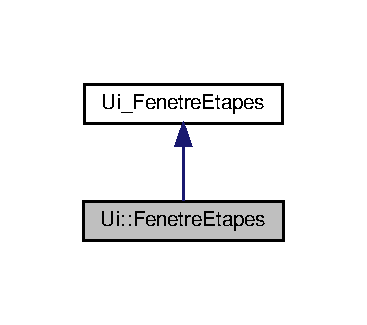
\includegraphics[width=176pt]{class_ui_1_1_fenetre_etapes__inherit__graph}
\end{center}
\end{figure}


Graphe de collaboration de Ui\+:\+:Fenetre\+Etapes\+:
\nopagebreak
\begin{figure}[H]
\begin{center}
\leavevmode
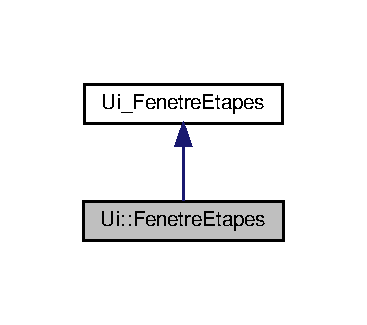
\includegraphics[width=176pt]{class_ui_1_1_fenetre_etapes__coll__graph}
\end{center}
\end{figure}
\subsection*{Membres hérités additionnels}


La documentation de cette classe a été générée à partir du fichier suivant \+:\begin{DoxyCompactItemize}
\item 
Lecteur\+Recette/\hyperlink{ui__etapes_8h}{ui\+\_\+etapes.\+h}\end{DoxyCompactItemize}

\hypertarget{class_ui_1_1_fenetre_presentation}{}\section{Référence de la classe Ui\+:\+:Fenetre\+Presentation}
\label{class_ui_1_1_fenetre_presentation}\index{Ui\+::\+Fenetre\+Presentation@{Ui\+::\+Fenetre\+Presentation}}


{\ttfamily \#include $<$ui\+\_\+presentation.\+h$>$}



Graphe d\textquotesingle{}héritage de Ui\+:\+:Fenetre\+Presentation\+:
\nopagebreak
\begin{figure}[H]
\begin{center}
\leavevmode
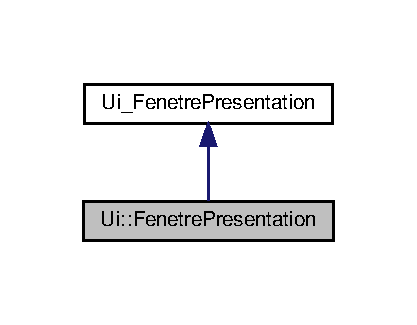
\includegraphics[width=206pt]{class_ui_1_1_fenetre_presentation__inherit__graph}
\end{center}
\end{figure}


Graphe de collaboration de Ui\+:\+:Fenetre\+Presentation\+:
\nopagebreak
\begin{figure}[H]
\begin{center}
\leavevmode
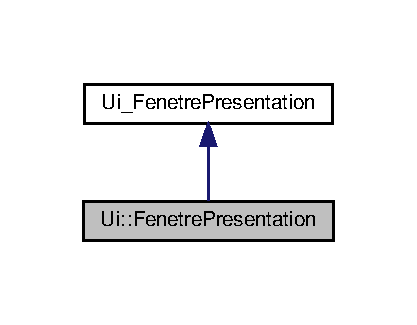
\includegraphics[width=206pt]{class_ui_1_1_fenetre_presentation__coll__graph}
\end{center}
\end{figure}
\subsection*{Membres hérités additionnels}


La documentation de cette classe a été générée à partir du fichier suivant \+:\begin{DoxyCompactItemize}
\item 
Lecteur\+Recette/\hyperlink{ui__presentation_8h}{ui\+\_\+presentation.\+h}\end{DoxyCompactItemize}

\hypertarget{class_lecteur_json}{}\section{Référence de la classe Lecteur\+Json}
\label{class_lecteur_json}\index{Lecteur\+Json@{Lecteur\+Json}}


Classe qui permet la lecture d\textquotesingle{}un fichier J\+S\+ON.  




{\ttfamily \#include $<$lecteurjson.\+h$>$}



Graphe de collaboration de Lecteur\+Json\+:
\nopagebreak
\begin{figure}[H]
\begin{center}
\leavevmode
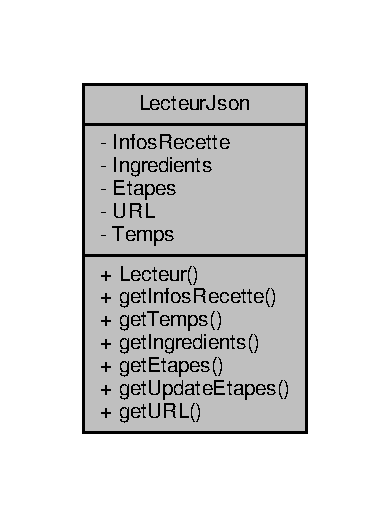
\includegraphics[width=187pt]{class_lecteur_json__coll__graph}
\end{center}
\end{figure}
\subsection*{Fonctions membres publiques}
\begin{DoxyCompactItemize}
\item 
void \hyperlink{class_lecteur_json_a6b74dbecd8cb87168fb2d36bc1a22f2b}{Lecteur} (Q\+String)
\begin{DoxyCompactList}\small\item\em Fonction qui extrait les différentes infos du fichier Json. \end{DoxyCompactList}\item 
Q\+String\+List \hyperlink{class_lecteur_json_a0c507870050e16de3688d310d1f3b65a}{get\+Infos\+Recette} ()
\item 
Q\+String\+List \hyperlink{class_lecteur_json_a88d73523c1775a8c7001b5abae152740}{get\+Temps} ()
\item 
Q\+String\+List \hyperlink{class_lecteur_json_a0c18d502de54aea85b4d76f1b2858423}{get\+Ingredients} ()
\item 
Q\+String\+List \hyperlink{class_lecteur_json_ab698142bf586bb224c35962525ce3915}{get\+Etapes} ()
\item 
Q\+String \hyperlink{class_lecteur_json_ad3a86b8dc577d1e6d77a66b8ece8442a}{get\+Update\+Etapes} (int i)
\item 
Q\+String\+List \hyperlink{class_lecteur_json_a4ceacda970b2b838bb41211decdd799f}{get\+U\+RL} ()
\end{DoxyCompactItemize}
\subsection*{Attributs privés}
\begin{DoxyCompactItemize}
\item 
Q\+String\+List \hyperlink{class_lecteur_json_a567a5bb99e9883f7906a89a46e322495}{Infos\+Recette}
\item 
Q\+String\+List \hyperlink{class_lecteur_json_a0648021cfe10db3555625e63c14961f9}{Ingredients}
\item 
Q\+String\+List \hyperlink{class_lecteur_json_a9328054d9a7e7f446cb047cab54c7b45}{Etapes}
\item 
Q\+String\+List \hyperlink{class_lecteur_json_ac4e3585c5c083c669273346ac6910353}{U\+RL}
\item 
Q\+String\+List \hyperlink{class_lecteur_json_a46972b215d8f7d30f68e7cf9c5711fc1}{Temps}
\end{DoxyCompactItemize}


\subsection{Description détaillée}
Classe qui permet la lecture d\textquotesingle{}un fichier J\+S\+ON. 

\subsection{Documentation des fonctions membres}
\mbox{\Hypertarget{class_lecteur_json_ab698142bf586bb224c35962525ce3915}\label{class_lecteur_json_ab698142bf586bb224c35962525ce3915}} 
\index{Lecteur\+Json@{Lecteur\+Json}!get\+Etapes@{get\+Etapes}}
\index{get\+Etapes@{get\+Etapes}!Lecteur\+Json@{Lecteur\+Json}}
\subsubsection{\texorpdfstring{get\+Etapes()}{getEtapes()}}
{\footnotesize\ttfamily Q\+String\+List Lecteur\+Json\+::get\+Etapes (\begin{DoxyParamCaption}{ }\end{DoxyParamCaption})\hspace{0.3cm}{\ttfamily [inline]}}

Q\+String\+List qui retourne les étapes de la recette Voici le graphe des appelants de cette fonction \+:
\nopagebreak
\begin{figure}[H]
\begin{center}
\leavevmode
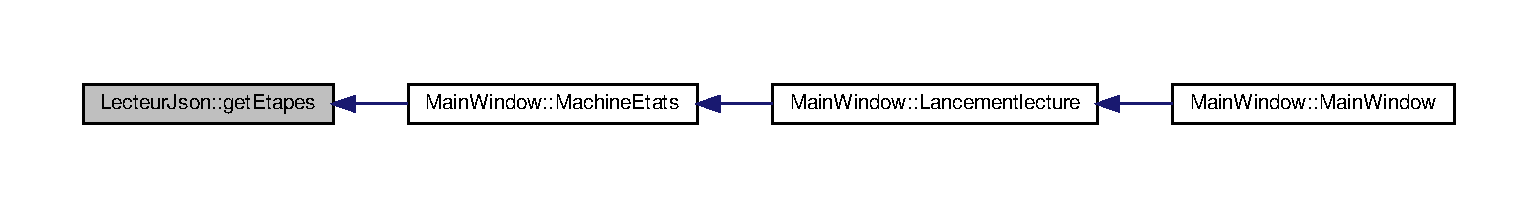
\includegraphics[width=350pt]{class_lecteur_json_ab698142bf586bb224c35962525ce3915_icgraph}
\end{center}
\end{figure}
\mbox{\Hypertarget{class_lecteur_json_a0c507870050e16de3688d310d1f3b65a}\label{class_lecteur_json_a0c507870050e16de3688d310d1f3b65a}} 
\index{Lecteur\+Json@{Lecteur\+Json}!get\+Infos\+Recette@{get\+Infos\+Recette}}
\index{get\+Infos\+Recette@{get\+Infos\+Recette}!Lecteur\+Json@{Lecteur\+Json}}
\subsubsection{\texorpdfstring{get\+Infos\+Recette()}{getInfosRecette()}}
{\footnotesize\ttfamily Q\+String\+List Lecteur\+Json\+::get\+Infos\+Recette (\begin{DoxyParamCaption}{ }\end{DoxyParamCaption})\hspace{0.3cm}{\ttfamily [inline]}}

Q\+String\+List qui retourne les infos de la recette Voici le graphe des appelants de cette fonction \+:
\nopagebreak
\begin{figure}[H]
\begin{center}
\leavevmode
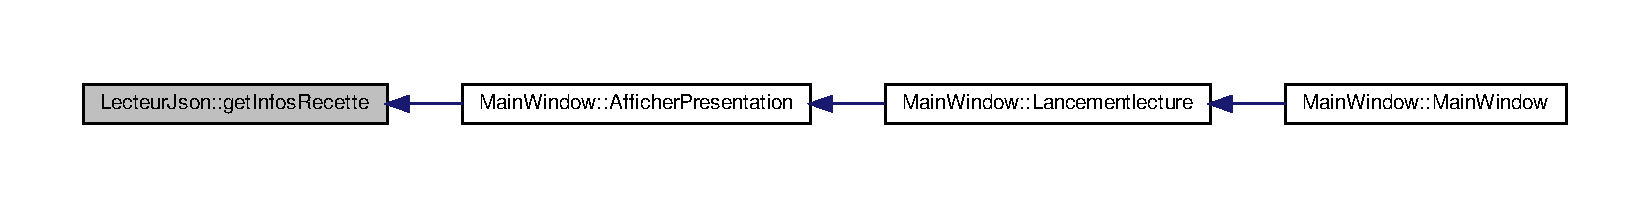
\includegraphics[width=350pt]{class_lecteur_json_a0c507870050e16de3688d310d1f3b65a_icgraph}
\end{center}
\end{figure}
\mbox{\Hypertarget{class_lecteur_json_a0c18d502de54aea85b4d76f1b2858423}\label{class_lecteur_json_a0c18d502de54aea85b4d76f1b2858423}} 
\index{Lecteur\+Json@{Lecteur\+Json}!get\+Ingredients@{get\+Ingredients}}
\index{get\+Ingredients@{get\+Ingredients}!Lecteur\+Json@{Lecteur\+Json}}
\subsubsection{\texorpdfstring{get\+Ingredients()}{getIngredients()}}
{\footnotesize\ttfamily Q\+String\+List Lecteur\+Json\+::get\+Ingredients (\begin{DoxyParamCaption}{ }\end{DoxyParamCaption})\hspace{0.3cm}{\ttfamily [inline]}}

Q\+String\+List qui retourne les ingredients de la recette Voici le graphe des appelants de cette fonction \+:
\nopagebreak
\begin{figure}[H]
\begin{center}
\leavevmode
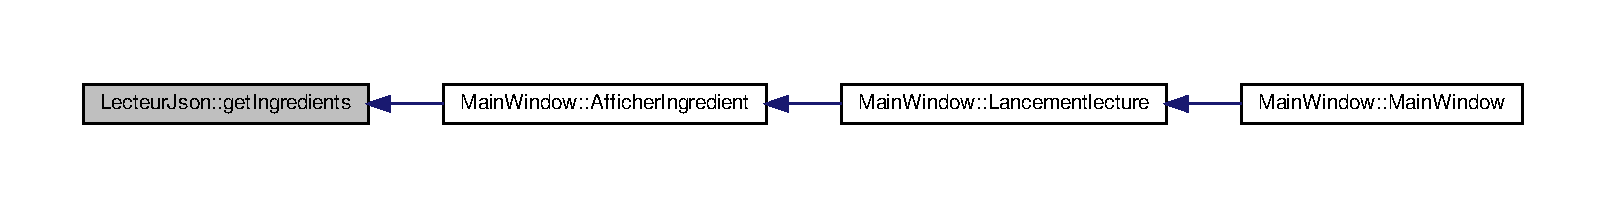
\includegraphics[width=350pt]{class_lecteur_json_a0c18d502de54aea85b4d76f1b2858423_icgraph}
\end{center}
\end{figure}
\mbox{\Hypertarget{class_lecteur_json_a88d73523c1775a8c7001b5abae152740}\label{class_lecteur_json_a88d73523c1775a8c7001b5abae152740}} 
\index{Lecteur\+Json@{Lecteur\+Json}!get\+Temps@{get\+Temps}}
\index{get\+Temps@{get\+Temps}!Lecteur\+Json@{Lecteur\+Json}}
\subsubsection{\texorpdfstring{get\+Temps()}{getTemps()}}
{\footnotesize\ttfamily Q\+String\+List Lecteur\+Json\+::get\+Temps (\begin{DoxyParamCaption}{ }\end{DoxyParamCaption})\hspace{0.3cm}{\ttfamily [inline]}}

Q\+String\+List qui retourne les temps de la recette Voici le graphe des appelants de cette fonction \+:
\nopagebreak
\begin{figure}[H]
\begin{center}
\leavevmode
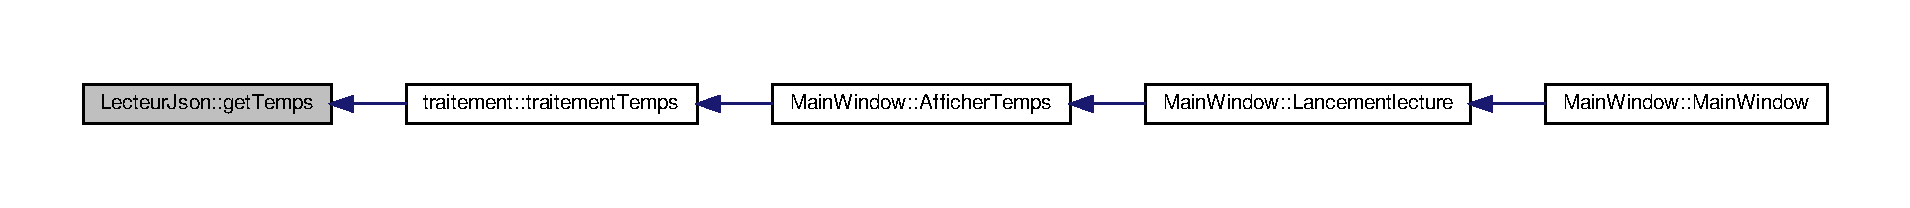
\includegraphics[width=350pt]{class_lecteur_json_a88d73523c1775a8c7001b5abae152740_icgraph}
\end{center}
\end{figure}
\mbox{\Hypertarget{class_lecteur_json_ad3a86b8dc577d1e6d77a66b8ece8442a}\label{class_lecteur_json_ad3a86b8dc577d1e6d77a66b8ece8442a}} 
\index{Lecteur\+Json@{Lecteur\+Json}!get\+Update\+Etapes@{get\+Update\+Etapes}}
\index{get\+Update\+Etapes@{get\+Update\+Etapes}!Lecteur\+Json@{Lecteur\+Json}}
\subsubsection{\texorpdfstring{get\+Update\+Etapes()}{getUpdateEtapes()}}
{\footnotesize\ttfamily Q\+String Lecteur\+Json\+::get\+Update\+Etapes (\begin{DoxyParamCaption}\item[{int}]{i }\end{DoxyParamCaption})\hspace{0.3cm}{\ttfamily [inline]}}

Q\+String qui retourne le numéro de l\textquotesingle{}étape Voici le graphe des appelants de cette fonction \+:
\nopagebreak
\begin{figure}[H]
\begin{center}
\leavevmode
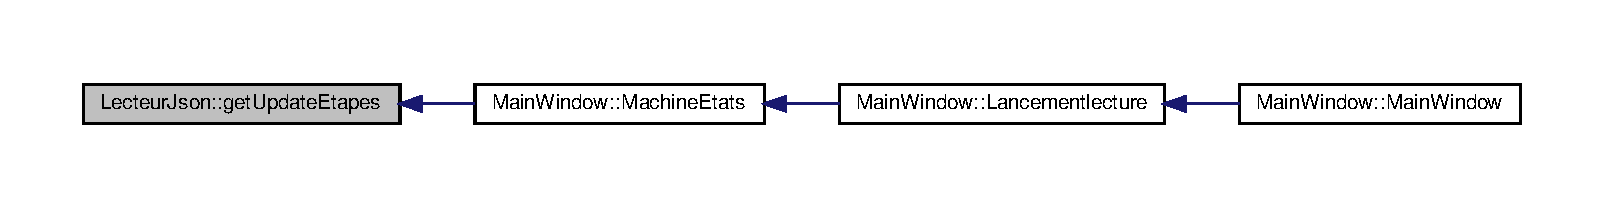
\includegraphics[width=350pt]{class_lecteur_json_ad3a86b8dc577d1e6d77a66b8ece8442a_icgraph}
\end{center}
\end{figure}
\mbox{\Hypertarget{class_lecteur_json_a4ceacda970b2b838bb41211decdd799f}\label{class_lecteur_json_a4ceacda970b2b838bb41211decdd799f}} 
\index{Lecteur\+Json@{Lecteur\+Json}!get\+U\+RL@{get\+U\+RL}}
\index{get\+U\+RL@{get\+U\+RL}!Lecteur\+Json@{Lecteur\+Json}}
\subsubsection{\texorpdfstring{get\+U\+R\+L()}{getURL()}}
{\footnotesize\ttfamily Q\+String\+List Lecteur\+Json\+::get\+U\+RL (\begin{DoxyParamCaption}{ }\end{DoxyParamCaption})\hspace{0.3cm}{\ttfamily [inline]}}

Q\+String\+List qui retourne l\textquotesingle{}U\+RL de la recette Voici le graphe des appelants de cette fonction \+:
\nopagebreak
\begin{figure}[H]
\begin{center}
\leavevmode
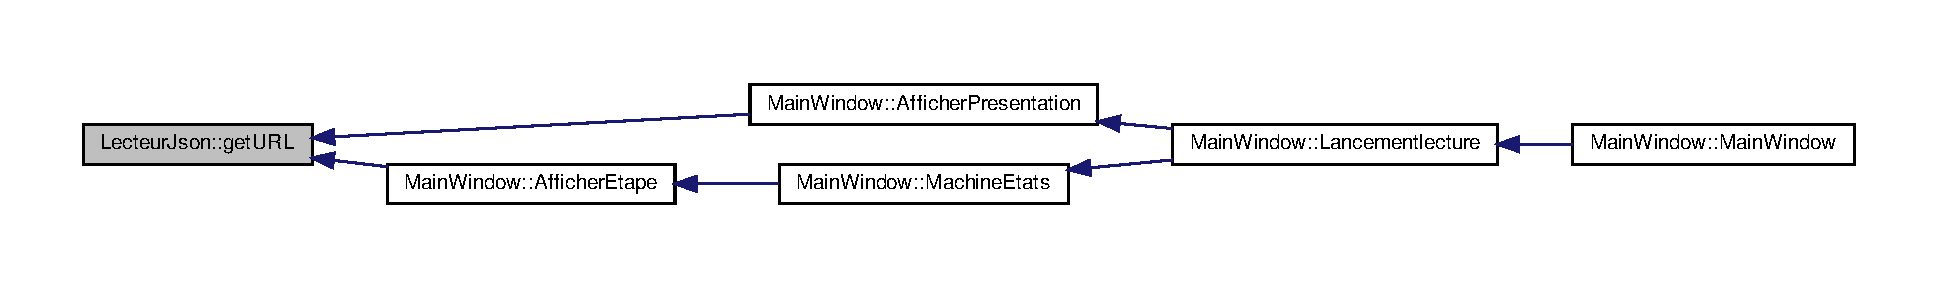
\includegraphics[width=350pt]{class_lecteur_json_a4ceacda970b2b838bb41211decdd799f_icgraph}
\end{center}
\end{figure}
\mbox{\Hypertarget{class_lecteur_json_a6b74dbecd8cb87168fb2d36bc1a22f2b}\label{class_lecteur_json_a6b74dbecd8cb87168fb2d36bc1a22f2b}} 
\index{Lecteur\+Json@{Lecteur\+Json}!Lecteur@{Lecteur}}
\index{Lecteur@{Lecteur}!Lecteur\+Json@{Lecteur\+Json}}
\subsubsection{\texorpdfstring{Lecteur()}{Lecteur()}}
{\footnotesize\ttfamily Lecteur\+Json\+::\+Lecteur (\begin{DoxyParamCaption}\item[{Q\+String}]{nom\+Fichier }\end{DoxyParamCaption})}



Fonction qui extrait les différentes infos du fichier Json. 

Fonction qui lit le fichier Json.


\begin{DoxyParams}{Paramètres}
{\em Q\+String} & qui contient le chemin du fichier. \\
\hline
\end{DoxyParams}
Voici le graphe des appelants de cette fonction \+:
\nopagebreak
\begin{figure}[H]
\begin{center}
\leavevmode
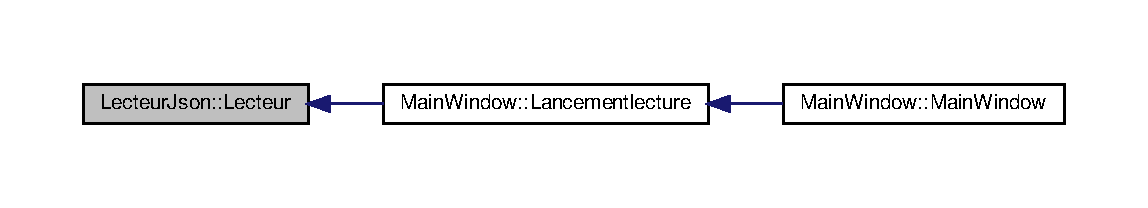
\includegraphics[width=350pt]{class_lecteur_json_a6b74dbecd8cb87168fb2d36bc1a22f2b_icgraph}
\end{center}
\end{figure}


\subsection{Documentation des données membres}
\mbox{\Hypertarget{class_lecteur_json_a9328054d9a7e7f446cb047cab54c7b45}\label{class_lecteur_json_a9328054d9a7e7f446cb047cab54c7b45}} 
\index{Lecteur\+Json@{Lecteur\+Json}!Etapes@{Etapes}}
\index{Etapes@{Etapes}!Lecteur\+Json@{Lecteur\+Json}}
\subsubsection{\texorpdfstring{Etapes}{Etapes}}
{\footnotesize\ttfamily Q\+String\+List Lecteur\+Json\+::\+Etapes\hspace{0.3cm}{\ttfamily [private]}}

\mbox{\Hypertarget{class_lecteur_json_a567a5bb99e9883f7906a89a46e322495}\label{class_lecteur_json_a567a5bb99e9883f7906a89a46e322495}} 
\index{Lecteur\+Json@{Lecteur\+Json}!Infos\+Recette@{Infos\+Recette}}
\index{Infos\+Recette@{Infos\+Recette}!Lecteur\+Json@{Lecteur\+Json}}
\subsubsection{\texorpdfstring{Infos\+Recette}{InfosRecette}}
{\footnotesize\ttfamily Q\+String\+List Lecteur\+Json\+::\+Infos\+Recette\hspace{0.3cm}{\ttfamily [private]}}

\mbox{\Hypertarget{class_lecteur_json_a0648021cfe10db3555625e63c14961f9}\label{class_lecteur_json_a0648021cfe10db3555625e63c14961f9}} 
\index{Lecteur\+Json@{Lecteur\+Json}!Ingredients@{Ingredients}}
\index{Ingredients@{Ingredients}!Lecteur\+Json@{Lecteur\+Json}}
\subsubsection{\texorpdfstring{Ingredients}{Ingredients}}
{\footnotesize\ttfamily Q\+String\+List Lecteur\+Json\+::\+Ingredients\hspace{0.3cm}{\ttfamily [private]}}

\mbox{\Hypertarget{class_lecteur_json_a46972b215d8f7d30f68e7cf9c5711fc1}\label{class_lecteur_json_a46972b215d8f7d30f68e7cf9c5711fc1}} 
\index{Lecteur\+Json@{Lecteur\+Json}!Temps@{Temps}}
\index{Temps@{Temps}!Lecteur\+Json@{Lecteur\+Json}}
\subsubsection{\texorpdfstring{Temps}{Temps}}
{\footnotesize\ttfamily Q\+String\+List Lecteur\+Json\+::\+Temps\hspace{0.3cm}{\ttfamily [private]}}

\mbox{\Hypertarget{class_lecteur_json_ac4e3585c5c083c669273346ac6910353}\label{class_lecteur_json_ac4e3585c5c083c669273346ac6910353}} 
\index{Lecteur\+Json@{Lecteur\+Json}!U\+RL@{U\+RL}}
\index{U\+RL@{U\+RL}!Lecteur\+Json@{Lecteur\+Json}}
\subsubsection{\texorpdfstring{U\+RL}{URL}}
{\footnotesize\ttfamily Q\+String\+List Lecteur\+Json\+::\+U\+RL\hspace{0.3cm}{\ttfamily [private]}}



La documentation de cette classe a été générée à partir des fichiers suivants \+:\begin{DoxyCompactItemize}
\item 
Lecteur\+Recette/\hyperlink{lecteurjson_8h}{lecteurjson.\+h}\item 
Lecteur\+Recette/\hyperlink{_lecteur_json_8cpp}{Lecteur\+Json.\+cpp}\end{DoxyCompactItemize}

\hypertarget{class_main_window}{}\section{Main\+Window Class Reference}
\label{class_main_window}\index{Main\+Window@{Main\+Window}}


classe qui gère l\textquotesingle{}affichage des différentes fenêtres  




{\ttfamily \#include $<$mainwindow.\+h$>$}



Inheritance diagram for Main\+Window\+:
\nopagebreak
\begin{figure}[H]
\begin{center}
\leavevmode
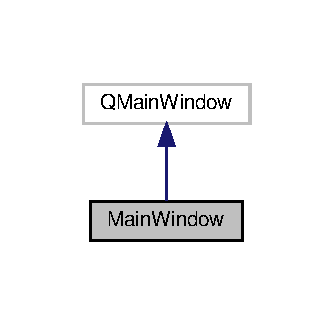
\includegraphics[width=160pt]{class_main_window__inherit__graph}
\end{center}
\end{figure}


Collaboration diagram for Main\+Window\+:
\nopagebreak
\begin{figure}[H]
\begin{center}
\leavevmode
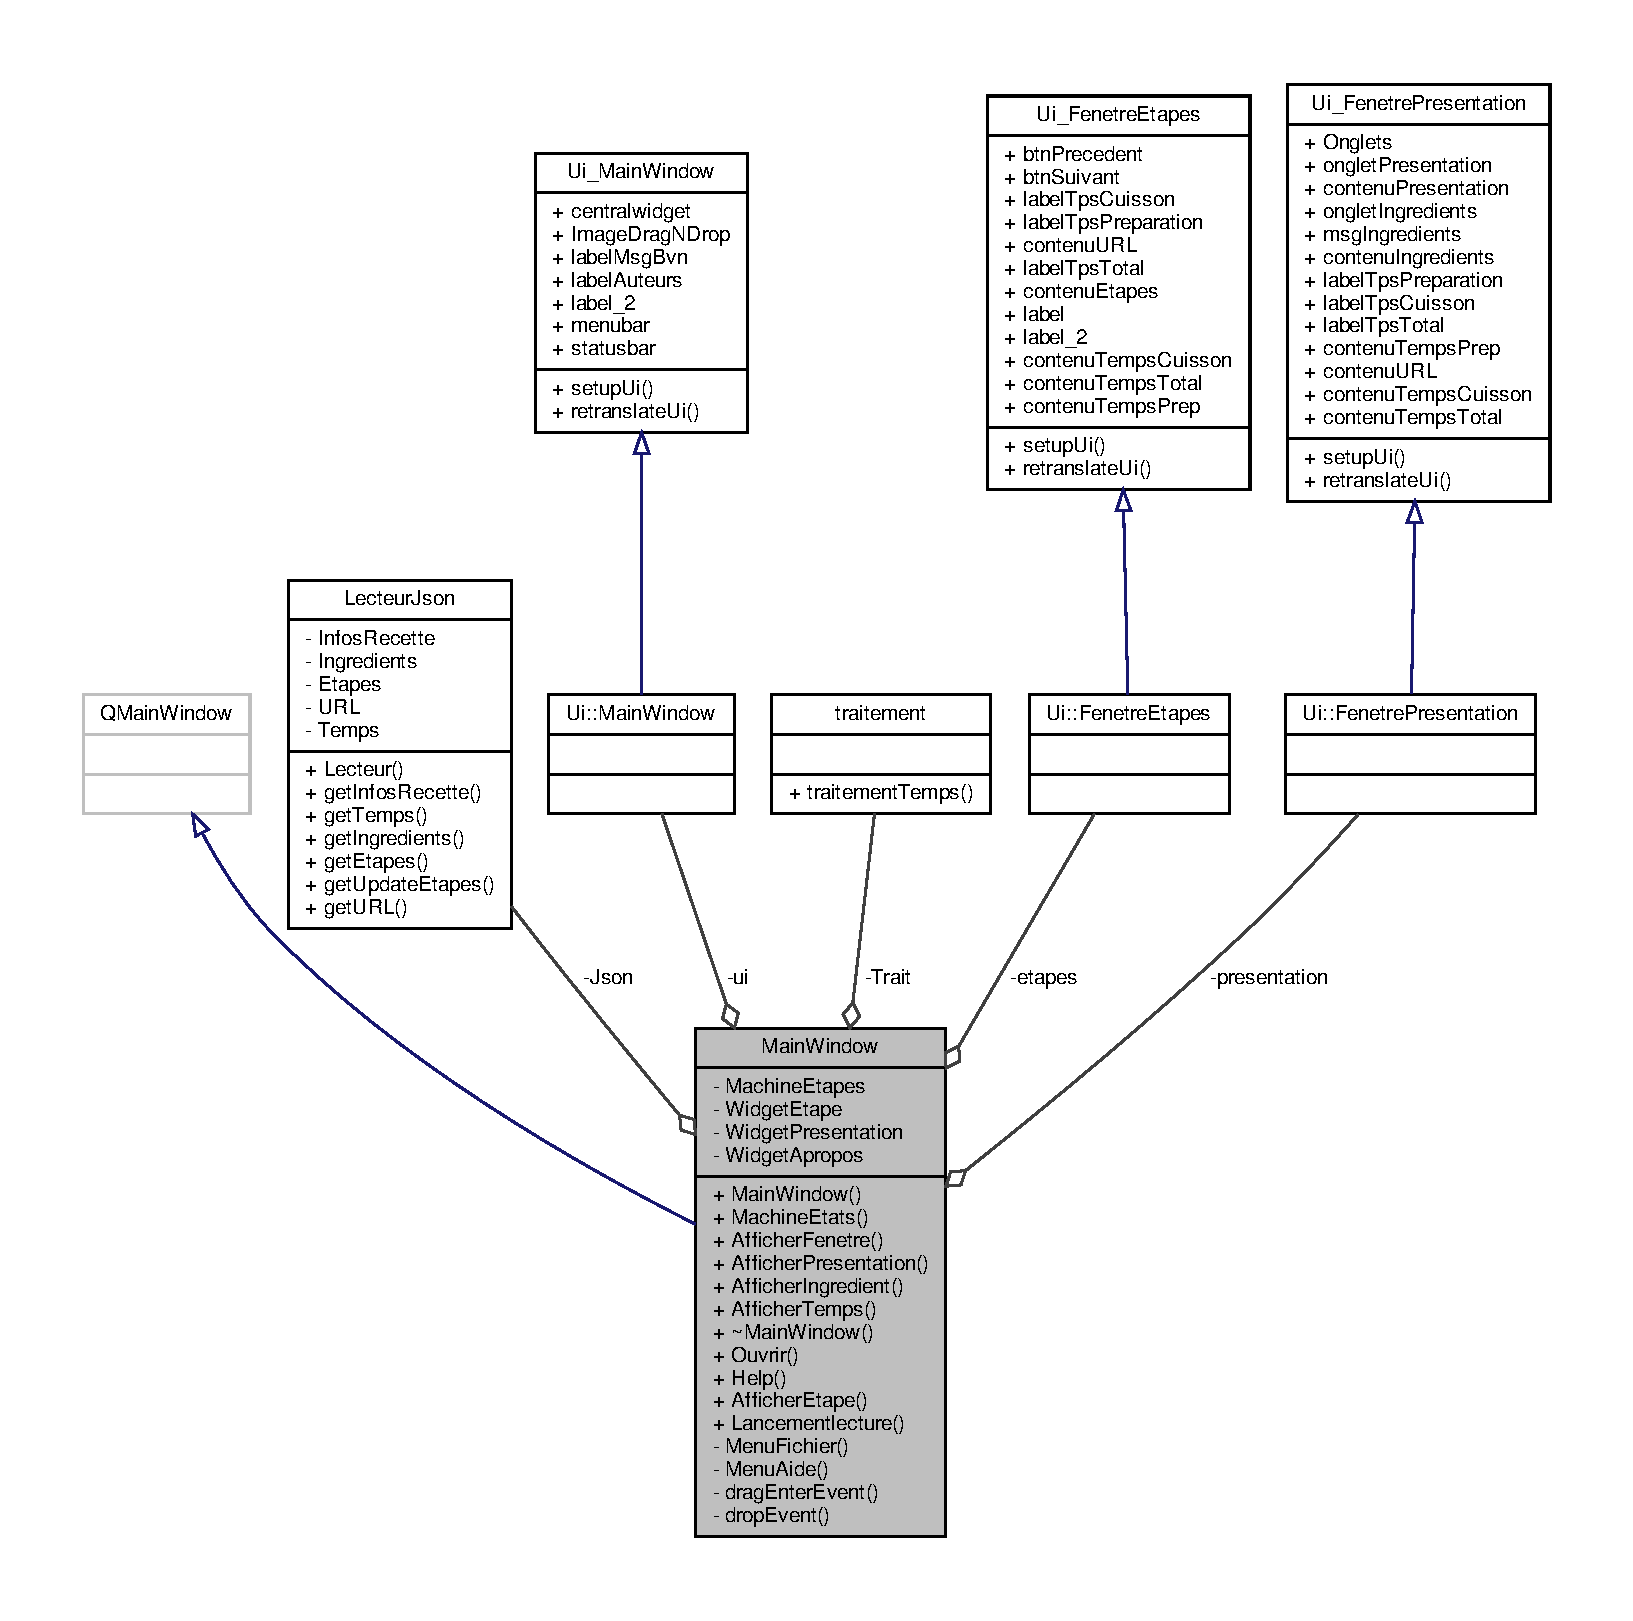
\includegraphics[width=160pt]{class_main_window__coll__graph}
\end{center}
\end{figure}
\subsection*{Public Slots}
\begin{DoxyCompactItemize}
\item 
void \hyperlink{class_main_window_a37a30280ba05a52445ecbea9deaa5385}{Ouvrir} (const Q\+String \&path=Q\+String())
\begin{DoxyCompactList}\small\item\em Fonction qui permet d\textquotesingle{}ouvrir un fichier sur la fenêtre. \end{DoxyCompactList}\item 
void \hyperlink{class_main_window_a25ec89113c14218717cfade9a58f8fdb}{Help} ()
\begin{DoxyCompactList}\small\item\em Menu aide sur la fenêtre principal. \end{DoxyCompactList}\item 
void \hyperlink{class_main_window_ae90cd3ee3e8e0b2ddf842514fafd13dc}{Afficher\+Etape} ()
\begin{DoxyCompactList}\small\item\em Fonction qui affiche les etapes de la recette. \end{DoxyCompactList}\item 
void \hyperlink{class_main_window_ac368dfd7e2609f0cb72fc1428771aa97}{Lancementlecture} (Q\+String)
\begin{DoxyCompactList}\small\item\em Fonction qui appelle la fonction qui traite le json + affiche toutes les informations nécessaires. \end{DoxyCompactList}\end{DoxyCompactItemize}
\subsection*{Signals}
\begin{DoxyCompactItemize}
\item 
void \hyperlink{class_main_window_a397116dafcb548fec351091cc025b822}{chemin\+Fichier} (Q\+String)
\begin{DoxyCompactList}\small\item\em Signal qui indique qu\textquotesingle{}un fichier à été trouvé \end{DoxyCompactList}\item 
void \hyperlink{class_main_window_a9a0c33e6e696ffc763560205f992650d}{Clear\+Label} ()
\begin{DoxyCompactList}\small\item\em Signal qui clear les numéro des étapes. \end{DoxyCompactList}\end{DoxyCompactItemize}
\subsection*{Public Member Functions}
\begin{DoxyCompactItemize}
\item 
\hyperlink{class_main_window_a996c5a2b6f77944776856f08ec30858d}{Main\+Window} (Q\+Widget $\ast$parent=nullptr)
\begin{DoxyCompactList}\small\item\em Constructeur de la classe \hyperlink{class_main_window}{Main\+Window}. \end{DoxyCompactList}\item 
void \hyperlink{class_main_window_a59cd9a83e43405ae1ad5c18e79b04db5}{Machine\+Etats} ()
\item 
void \hyperlink{class_main_window_aad6ceb17a20cccdc88050996600e9616}{Afficher\+Fenetre} ()
\begin{DoxyCompactList}\small\item\em Afficher Fenêtre. \end{DoxyCompactList}\item 
void \hyperlink{class_main_window_aeddbbb22621e412b4749d331c1d45001}{Afficher\+Presentation} ()
\begin{DoxyCompactList}\small\item\em Afficher Présentation. \end{DoxyCompactList}\item 
void \hyperlink{class_main_window_ad4059abf16eb904f988371b3791002bf}{Afficher\+Ingredient} ()
\begin{DoxyCompactList}\small\item\em Afficher Ingrédient. \end{DoxyCompactList}\item 
void \hyperlink{class_main_window_a33811a52abf8f1ce71ec4e150d9c9ac8}{Afficher\+Temps} ()
\begin{DoxyCompactList}\small\item\em Afficher temps. \end{DoxyCompactList}\item 
\hyperlink{class_main_window_ae98d00a93bc118200eeef9f9bba1dba7}{$\sim$\+Main\+Window} ()
\begin{DoxyCompactList}\small\item\em Destructeur. \end{DoxyCompactList}\end{DoxyCompactItemize}


\subsection{Detailed Description}
classe qui gère l\textquotesingle{}affichage des différentes fenêtres 

\subsection{Constructor \& Destructor Documentation}
\mbox{\Hypertarget{class_main_window_a996c5a2b6f77944776856f08ec30858d}\label{class_main_window_a996c5a2b6f77944776856f08ec30858d}} 
\index{Main\+Window@{Main\+Window}!Main\+Window@{Main\+Window}}
\index{Main\+Window@{Main\+Window}!Main\+Window@{Main\+Window}}
\subsubsection{\texorpdfstring{Main\+Window()}{MainWindow()}}
{\footnotesize\ttfamily Main\+Window\+::\+Main\+Window (\begin{DoxyParamCaption}\item[{Q\+Widget $\ast$}]{parent = {\ttfamily nullptr} }\end{DoxyParamCaption})}



Constructeur de la classe \hyperlink{class_main_window}{Main\+Window}. 


\begin{DoxyParams}{Parameters}
{\em parent} & Pointeur sur Q\+Widget \\
\hline
\end{DoxyParams}
\mbox{\Hypertarget{class_main_window_ae98d00a93bc118200eeef9f9bba1dba7}\label{class_main_window_ae98d00a93bc118200eeef9f9bba1dba7}} 
\index{Main\+Window@{Main\+Window}!````~Main\+Window@{$\sim$\+Main\+Window}}
\index{````~Main\+Window@{$\sim$\+Main\+Window}!Main\+Window@{Main\+Window}}
\subsubsection{\texorpdfstring{$\sim$\+Main\+Window()}{~MainWindow()}}
{\footnotesize\ttfamily Main\+Window\+::$\sim$\+Main\+Window (\begin{DoxyParamCaption}{ }\end{DoxyParamCaption})}



Destructeur. 

Destructeur de la classe \hyperlink{class_main_window}{Main\+Window} 

\subsection{Member Function Documentation}
\mbox{\Hypertarget{class_main_window_ae90cd3ee3e8e0b2ddf842514fafd13dc}\label{class_main_window_ae90cd3ee3e8e0b2ddf842514fafd13dc}} 
\index{Main\+Window@{Main\+Window}!Afficher\+Etape@{Afficher\+Etape}}
\index{Afficher\+Etape@{Afficher\+Etape}!Main\+Window@{Main\+Window}}
\subsubsection{\texorpdfstring{Afficher\+Etape}{AfficherEtape}}
{\footnotesize\ttfamily Main\+Window\+::\+Afficher\+Etape (\begin{DoxyParamCaption}{ }\end{DoxyParamCaption})\hspace{0.3cm}{\ttfamily [slot]}}



Fonction qui affiche les etapes de la recette. 

\mbox{\Hypertarget{class_main_window_aad6ceb17a20cccdc88050996600e9616}\label{class_main_window_aad6ceb17a20cccdc88050996600e9616}} 
\index{Main\+Window@{Main\+Window}!Afficher\+Fenetre@{Afficher\+Fenetre}}
\index{Afficher\+Fenetre@{Afficher\+Fenetre}!Main\+Window@{Main\+Window}}
\subsubsection{\texorpdfstring{Afficher\+Fenetre()}{AfficherFenetre()}}
{\footnotesize\ttfamily void Main\+Window\+::\+Afficher\+Fenetre (\begin{DoxyParamCaption}{ }\end{DoxyParamCaption})}



Afficher Fenêtre. 

Fonction Qui affichee les fenêtres après lecture du J\+S\+ON. \mbox{\Hypertarget{class_main_window_ad4059abf16eb904f988371b3791002bf}\label{class_main_window_ad4059abf16eb904f988371b3791002bf}} 
\index{Main\+Window@{Main\+Window}!Afficher\+Ingredient@{Afficher\+Ingredient}}
\index{Afficher\+Ingredient@{Afficher\+Ingredient}!Main\+Window@{Main\+Window}}
\subsubsection{\texorpdfstring{Afficher\+Ingredient()}{AfficherIngredient()}}
{\footnotesize\ttfamily void Main\+Window\+::\+Afficher\+Ingredient (\begin{DoxyParamCaption}{ }\end{DoxyParamCaption})}



Afficher Ingrédient. 

Affiche les ingédients dans la fenêtre Ingredient après lecture du J\+S\+ON \mbox{\Hypertarget{class_main_window_aeddbbb22621e412b4749d331c1d45001}\label{class_main_window_aeddbbb22621e412b4749d331c1d45001}} 
\index{Main\+Window@{Main\+Window}!Afficher\+Presentation@{Afficher\+Presentation}}
\index{Afficher\+Presentation@{Afficher\+Presentation}!Main\+Window@{Main\+Window}}
\subsubsection{\texorpdfstring{Afficher\+Presentation()}{AfficherPresentation()}}
{\footnotesize\ttfamily void Main\+Window\+::\+Afficher\+Presentation (\begin{DoxyParamCaption}{ }\end{DoxyParamCaption})}



Afficher Présentation. 

Affiche le texte dans la fenêtre présentation après lecture du J\+S\+ON. \mbox{\Hypertarget{class_main_window_a33811a52abf8f1ce71ec4e150d9c9ac8}\label{class_main_window_a33811a52abf8f1ce71ec4e150d9c9ac8}} 
\index{Main\+Window@{Main\+Window}!Afficher\+Temps@{Afficher\+Temps}}
\index{Afficher\+Temps@{Afficher\+Temps}!Main\+Window@{Main\+Window}}
\subsubsection{\texorpdfstring{Afficher\+Temps()}{AfficherTemps()}}
{\footnotesize\ttfamily void Main\+Window\+::\+Afficher\+Temps (\begin{DoxyParamCaption}{ }\end{DoxyParamCaption})}



Afficher temps. 

Affiche le temp après traitement. \mbox{\Hypertarget{class_main_window_a397116dafcb548fec351091cc025b822}\label{class_main_window_a397116dafcb548fec351091cc025b822}} 
\index{Main\+Window@{Main\+Window}!chemin\+Fichier@{chemin\+Fichier}}
\index{chemin\+Fichier@{chemin\+Fichier}!Main\+Window@{Main\+Window}}
\subsubsection{\texorpdfstring{chemin\+Fichier}{cheminFichier}}
{\footnotesize\ttfamily void Main\+Window\+::chemin\+Fichier (\begin{DoxyParamCaption}\item[{Q\+String}]{ }\end{DoxyParamCaption})\hspace{0.3cm}{\ttfamily [signal]}}



Signal qui indique qu\textquotesingle{}un fichier à été trouvé 

\begin{DoxySeeAlso}{See also}
signal \hyperlink{class_main_window_a397116dafcb548fec351091cc025b822}{chemin\+Fichier} 
\end{DoxySeeAlso}

\begin{DoxyParams}{Parameters}
{\em Q\+String} & qui contient le chemin du fichier \\
\hline
\end{DoxyParams}
\mbox{\Hypertarget{class_main_window_a9a0c33e6e696ffc763560205f992650d}\label{class_main_window_a9a0c33e6e696ffc763560205f992650d}} 
\index{Main\+Window@{Main\+Window}!Clear\+Label@{Clear\+Label}}
\index{Clear\+Label@{Clear\+Label}!Main\+Window@{Main\+Window}}
\subsubsection{\texorpdfstring{Clear\+Label}{ClearLabel}}
{\footnotesize\ttfamily void Main\+Window\+::\+Clear\+Label (\begin{DoxyParamCaption}{ }\end{DoxyParamCaption})\hspace{0.3cm}{\ttfamily [signal]}}



Signal qui clear les numéro des étapes. 

\begin{DoxySeeAlso}{See also}
signal \hyperlink{class_main_window_a9a0c33e6e696ffc763560205f992650d}{Clear\+Label} 
\end{DoxySeeAlso}
\mbox{\Hypertarget{class_main_window_a25ec89113c14218717cfade9a58f8fdb}\label{class_main_window_a25ec89113c14218717cfade9a58f8fdb}} 
\index{Main\+Window@{Main\+Window}!Help@{Help}}
\index{Help@{Help}!Main\+Window@{Main\+Window}}
\subsubsection{\texorpdfstring{Help}{Help}}
{\footnotesize\ttfamily Main\+Window\+::\+Help (\begin{DoxyParamCaption}{ }\end{DoxyParamCaption})\hspace{0.3cm}{\ttfamily [slot]}}



Menu aide sur la fenêtre principal. 

\mbox{\Hypertarget{class_main_window_ac368dfd7e2609f0cb72fc1428771aa97}\label{class_main_window_ac368dfd7e2609f0cb72fc1428771aa97}} 
\index{Main\+Window@{Main\+Window}!Lancementlecture@{Lancementlecture}}
\index{Lancementlecture@{Lancementlecture}!Main\+Window@{Main\+Window}}
\subsubsection{\texorpdfstring{Lancementlecture}{Lancementlecture}}
{\footnotesize\ttfamily Main\+Window\+::\+Lancementlecture (\begin{DoxyParamCaption}\item[{Q\+String}]{nom\+Fichier }\end{DoxyParamCaption})\hspace{0.3cm}{\ttfamily [slot]}}



Fonction qui appelle la fonction qui traite le json + affiche toutes les informations nécessaires. 


\begin{DoxyParams}{Parameters}
{\em Q\+String} & qui contient le chemin du fichier(reçue par la fonction ouvrir). \\
\hline
\end{DoxyParams}
\mbox{\Hypertarget{class_main_window_a59cd9a83e43405ae1ad5c18e79b04db5}\label{class_main_window_a59cd9a83e43405ae1ad5c18e79b04db5}} 
\index{Main\+Window@{Main\+Window}!Machine\+Etats@{Machine\+Etats}}
\index{Machine\+Etats@{Machine\+Etats}!Main\+Window@{Main\+Window}}
\subsubsection{\texorpdfstring{Machine\+Etats()}{MachineEtats()}}
{\footnotesize\ttfamily void Main\+Window\+::\+Machine\+Etats (\begin{DoxyParamCaption}{ }\end{DoxyParamCaption})}

\mbox{\Hypertarget{class_main_window_a37a30280ba05a52445ecbea9deaa5385}\label{class_main_window_a37a30280ba05a52445ecbea9deaa5385}} 
\index{Main\+Window@{Main\+Window}!Ouvrir@{Ouvrir}}
\index{Ouvrir@{Ouvrir}!Main\+Window@{Main\+Window}}
\subsubsection{\texorpdfstring{Ouvrir}{Ouvrir}}
{\footnotesize\ttfamily Main\+Window\+::\+Ouvrir (\begin{DoxyParamCaption}\item[{const Q\+String \&}]{path = {\ttfamily QString()} }\end{DoxyParamCaption})\hspace{0.3cm}{\ttfamily [slot]}}



Fonction qui permet d\textquotesingle{}ouvrir un fichier sur la fenêtre. 


\begin{DoxyParams}{Parameters}
{\em Qstring} & qui contient le chemin du fichier. \\
\hline
\end{DoxyParams}


The documentation for this class was generated from the following files\+:\begin{DoxyCompactItemize}
\item 
\hyperlink{mainwindow_8h}{mainwindow.\+h}\item 
\hyperlink{mainwindow_8cpp}{mainwindow.\+cpp}\end{DoxyCompactItemize}

\hypertarget{class_ui_1_1_main_window}{}\section{Référence de la classe Ui\+:\+:Main\+Window}
\label{class_ui_1_1_main_window}\index{Ui\+::\+Main\+Window@{Ui\+::\+Main\+Window}}


{\ttfamily \#include $<$ui\+\_\+mainwindow.\+h$>$}



Graphe d\textquotesingle{}héritage de Ui\+:\+:Main\+Window\+:
\nopagebreak
\begin{figure}[H]
\begin{center}
\leavevmode
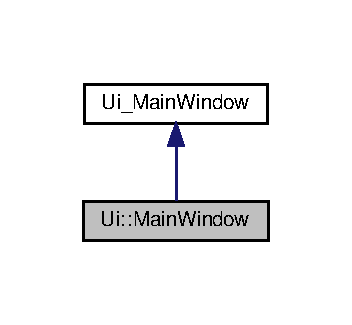
\includegraphics[width=169pt]{class_ui_1_1_main_window__inherit__graph}
\end{center}
\end{figure}


Graphe de collaboration de Ui\+:\+:Main\+Window\+:
\nopagebreak
\begin{figure}[H]
\begin{center}
\leavevmode
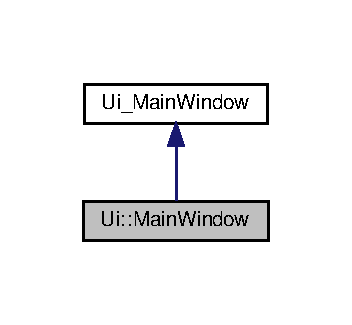
\includegraphics[width=169pt]{class_ui_1_1_main_window__coll__graph}
\end{center}
\end{figure}
\subsection*{Membres hérités additionnels}


La documentation de cette classe a été générée à partir du fichier suivant \+:\begin{DoxyCompactItemize}
\item 
Lecteur\+Recette/\hyperlink{ui__mainwindow_8h}{ui\+\_\+mainwindow.\+h}\end{DoxyCompactItemize}

\hypertarget{classtraitement}{}\section{traitement Class Reference}
\label{classtraitement}\index{traitement@{traitement}}


classe permettant le traitement du temps du fichier J\+Son  




{\ttfamily \#include $<$temps.\+h$>$}

\subsection*{Public Member Functions}
\begin{DoxyCompactItemize}
\item 
void \hyperlink{classtraitement_a2bc46fa58a25e3f3bf87dfc4fd08ebf8}{traitement\+Temps} (Q\+String\+List \&, Q\+String\+List \&, Q\+String\+List \&, \hyperlink{class_lecteur_json}{Lecteur\+Json})
\end{DoxyCompactItemize}


\subsection{Detailed Description}
classe permettant le traitement du temps du fichier J\+Son 

\subsection{Member Function Documentation}
\mbox{\Hypertarget{classtraitement_a2bc46fa58a25e3f3bf87dfc4fd08ebf8}\label{classtraitement_a2bc46fa58a25e3f3bf87dfc4fd08ebf8}} 
\index{traitement@{traitement}!traitement\+Temps@{traitement\+Temps}}
\index{traitement\+Temps@{traitement\+Temps}!traitement@{traitement}}
\subsubsection{\texorpdfstring{traitement\+Temps()}{traitementTemps()}}
{\footnotesize\ttfamily void traitement\+::traitement\+Temps (\begin{DoxyParamCaption}\item[{Q\+String\+List \&}]{contenu\+Temps\+Prep,  }\item[{Q\+String\+List \&}]{contenu\+Temps\+Cuisson,  }\item[{Q\+String\+List \&}]{contenu\+Temps\+Total,  }\item[{\hyperlink{class_lecteur_json}{Lecteur\+Json}}]{Json }\end{DoxyParamCaption})}



The documentation for this class was generated from the following files\+:\begin{DoxyCompactItemize}
\item 
\hyperlink{temps_8h}{temps.\+h}\item 
\hyperlink{temps_8cpp}{temps.\+cpp}\end{DoxyCompactItemize}

\hypertarget{class_ui___fenetre_etapes}{}\section{Référence de la classe Ui\+\_\+\+Fenetre\+Etapes}
\label{class_ui___fenetre_etapes}\index{Ui\+\_\+\+Fenetre\+Etapes@{Ui\+\_\+\+Fenetre\+Etapes}}


{\ttfamily \#include $<$ui\+\_\+etapes.\+h$>$}



Graphe d\textquotesingle{}héritage de Ui\+\_\+\+Fenetre\+Etapes\+:
\nopagebreak
\begin{figure}[H]
\begin{center}
\leavevmode
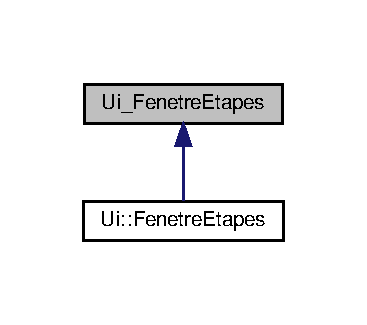
\includegraphics[width=206pt]{class_ui___fenetre_etapes__inherit__graph}
\end{center}
\end{figure}


Graphe de collaboration de Ui\+\_\+\+Fenetre\+Etapes\+:
\nopagebreak
\begin{figure}[H]
\begin{center}
\leavevmode
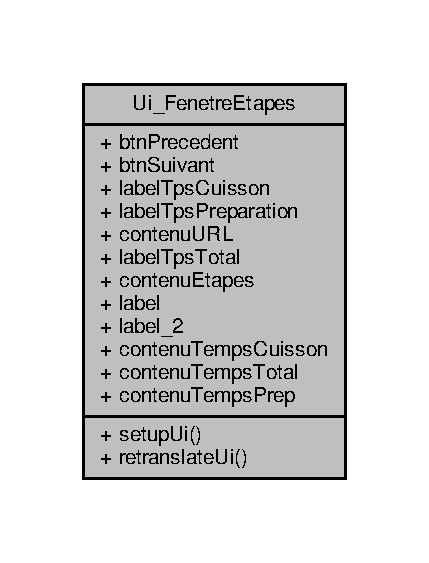
\includegraphics[width=206pt]{class_ui___fenetre_etapes__coll__graph}
\end{center}
\end{figure}
\subsection*{Fonctions membres publiques}
\begin{DoxyCompactItemize}
\item 
void \hyperlink{class_ui___fenetre_etapes_a5bf35503b72beb223e5a03ea046524a1}{setup\+Ui} (Q\+Widget $\ast$Fenetre\+Etapes)
\item 
void \hyperlink{class_ui___fenetre_etapes_a12b8a73438c7adfe883f9deb6af95426}{retranslate\+Ui} (Q\+Widget $\ast$Fenetre\+Etapes)
\end{DoxyCompactItemize}
\subsection*{Attributs publics}
\begin{DoxyCompactItemize}
\item 
Q\+Push\+Button $\ast$ \hyperlink{class_ui___fenetre_etapes_afd2c805beef4f8e6df60ba666e2d9e3e}{btn\+Precedent}
\item 
Q\+Push\+Button $\ast$ \hyperlink{class_ui___fenetre_etapes_ac4cd6163fd1066a242e7b2d7560317fa}{btn\+Suivant}
\item 
Q\+Label $\ast$ \hyperlink{class_ui___fenetre_etapes_a504cc9ecca60aa437626e850cae88c5b}{label\+Tps\+Cuisson}
\item 
Q\+Label $\ast$ \hyperlink{class_ui___fenetre_etapes_ab1994c36dbf7f67f539517c6431cb96b}{label\+Tps\+Preparation}
\item 
Q\+List\+View $\ast$ \hyperlink{class_ui___fenetre_etapes_aa24feeee1b3348435a83ec44571c5f25}{contenu\+U\+RL}
\item 
Q\+Label $\ast$ \hyperlink{class_ui___fenetre_etapes_a3c1c06d0dd2dde35c651ad430dc04bda}{label\+Tps\+Total}
\item 
Q\+List\+Widget $\ast$ \hyperlink{class_ui___fenetre_etapes_a5ca61918507e2eeef4e8e1d47467cc70}{contenu\+Etapes}
\item 
Q\+Label $\ast$ \hyperlink{class_ui___fenetre_etapes_a53eae32c579e7339b50f669828d704d3}{label}
\item 
Q\+Label $\ast$ \hyperlink{class_ui___fenetre_etapes_a58449e87895513ba9014273128385d91}{label\+\_\+2}
\item 
Q\+List\+View $\ast$ \hyperlink{class_ui___fenetre_etapes_a135f3f5bd01ce6b6305b2c5fac8300b7}{contenu\+Temps\+Cuisson}
\item 
Q\+List\+View $\ast$ \hyperlink{class_ui___fenetre_etapes_a408df57a10027aa8dc496185822b0f22}{contenu\+Temps\+Total}
\item 
Q\+List\+View $\ast$ \hyperlink{class_ui___fenetre_etapes_ab6a00c484db7168498bffe4e8ccc5547}{contenu\+Temps\+Prep}
\end{DoxyCompactItemize}


\subsection{Documentation des fonctions membres}
\mbox{\Hypertarget{class_ui___fenetre_etapes_a12b8a73438c7adfe883f9deb6af95426}\label{class_ui___fenetre_etapes_a12b8a73438c7adfe883f9deb6af95426}} 
\index{Ui\+\_\+\+Fenetre\+Etapes@{Ui\+\_\+\+Fenetre\+Etapes}!retranslate\+Ui@{retranslate\+Ui}}
\index{retranslate\+Ui@{retranslate\+Ui}!Ui\+\_\+\+Fenetre\+Etapes@{Ui\+\_\+\+Fenetre\+Etapes}}
\subsubsection{\texorpdfstring{retranslate\+Ui()}{retranslateUi()}}
{\footnotesize\ttfamily void Ui\+\_\+\+Fenetre\+Etapes\+::retranslate\+Ui (\begin{DoxyParamCaption}\item[{Q\+Widget $\ast$}]{Fenetre\+Etapes }\end{DoxyParamCaption})\hspace{0.3cm}{\ttfamily [inline]}}

Voici le graphe des appelants de cette fonction \+:
\nopagebreak
\begin{figure}[H]
\begin{center}
\leavevmode
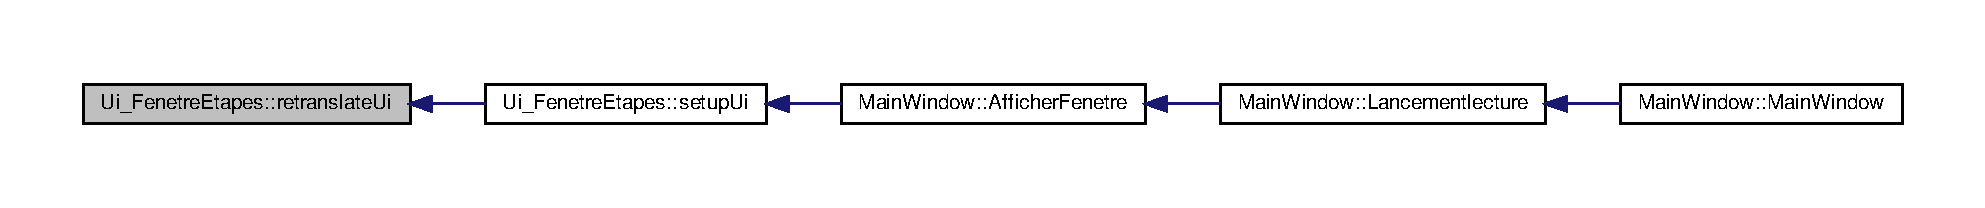
\includegraphics[width=350pt]{class_ui___fenetre_etapes_a12b8a73438c7adfe883f9deb6af95426_icgraph}
\end{center}
\end{figure}
\mbox{\Hypertarget{class_ui___fenetre_etapes_a5bf35503b72beb223e5a03ea046524a1}\label{class_ui___fenetre_etapes_a5bf35503b72beb223e5a03ea046524a1}} 
\index{Ui\+\_\+\+Fenetre\+Etapes@{Ui\+\_\+\+Fenetre\+Etapes}!setup\+Ui@{setup\+Ui}}
\index{setup\+Ui@{setup\+Ui}!Ui\+\_\+\+Fenetre\+Etapes@{Ui\+\_\+\+Fenetre\+Etapes}}
\subsubsection{\texorpdfstring{setup\+Ui()}{setupUi()}}
{\footnotesize\ttfamily void Ui\+\_\+\+Fenetre\+Etapes\+::setup\+Ui (\begin{DoxyParamCaption}\item[{Q\+Widget $\ast$}]{Fenetre\+Etapes }\end{DoxyParamCaption})\hspace{0.3cm}{\ttfamily [inline]}}

Voici le graphe d\textquotesingle{}appel pour cette fonction \+:
\nopagebreak
\begin{figure}[H]
\begin{center}
\leavevmode
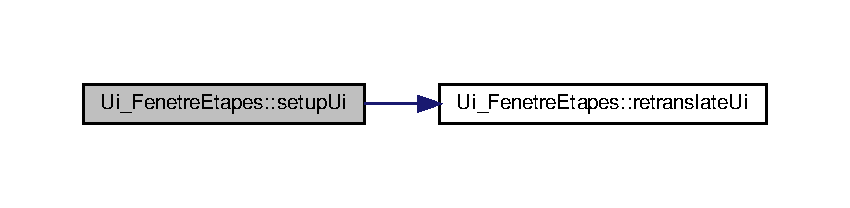
\includegraphics[width=350pt]{class_ui___fenetre_etapes_a5bf35503b72beb223e5a03ea046524a1_cgraph}
\end{center}
\end{figure}
Voici le graphe des appelants de cette fonction \+:
\nopagebreak
\begin{figure}[H]
\begin{center}
\leavevmode
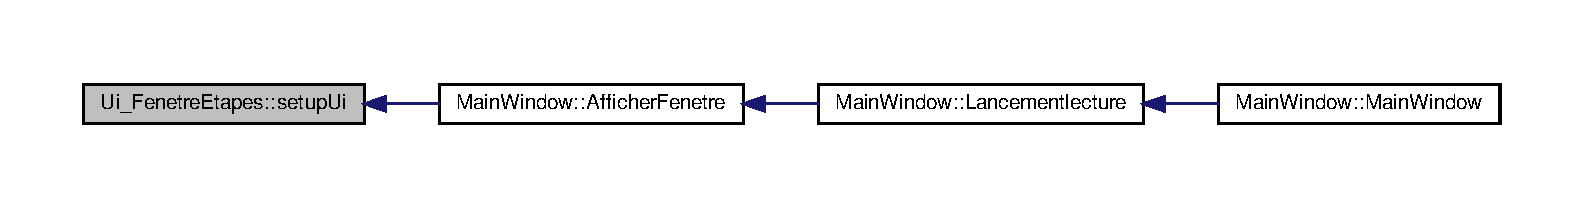
\includegraphics[width=350pt]{class_ui___fenetre_etapes_a5bf35503b72beb223e5a03ea046524a1_icgraph}
\end{center}
\end{figure}


\subsection{Documentation des données membres}
\mbox{\Hypertarget{class_ui___fenetre_etapes_afd2c805beef4f8e6df60ba666e2d9e3e}\label{class_ui___fenetre_etapes_afd2c805beef4f8e6df60ba666e2d9e3e}} 
\index{Ui\+\_\+\+Fenetre\+Etapes@{Ui\+\_\+\+Fenetre\+Etapes}!btn\+Precedent@{btn\+Precedent}}
\index{btn\+Precedent@{btn\+Precedent}!Ui\+\_\+\+Fenetre\+Etapes@{Ui\+\_\+\+Fenetre\+Etapes}}
\subsubsection{\texorpdfstring{btn\+Precedent}{btnPrecedent}}
{\footnotesize\ttfamily Q\+Push\+Button$\ast$ Ui\+\_\+\+Fenetre\+Etapes\+::btn\+Precedent}

\mbox{\Hypertarget{class_ui___fenetre_etapes_ac4cd6163fd1066a242e7b2d7560317fa}\label{class_ui___fenetre_etapes_ac4cd6163fd1066a242e7b2d7560317fa}} 
\index{Ui\+\_\+\+Fenetre\+Etapes@{Ui\+\_\+\+Fenetre\+Etapes}!btn\+Suivant@{btn\+Suivant}}
\index{btn\+Suivant@{btn\+Suivant}!Ui\+\_\+\+Fenetre\+Etapes@{Ui\+\_\+\+Fenetre\+Etapes}}
\subsubsection{\texorpdfstring{btn\+Suivant}{btnSuivant}}
{\footnotesize\ttfamily Q\+Push\+Button$\ast$ Ui\+\_\+\+Fenetre\+Etapes\+::btn\+Suivant}

\mbox{\Hypertarget{class_ui___fenetre_etapes_a5ca61918507e2eeef4e8e1d47467cc70}\label{class_ui___fenetre_etapes_a5ca61918507e2eeef4e8e1d47467cc70}} 
\index{Ui\+\_\+\+Fenetre\+Etapes@{Ui\+\_\+\+Fenetre\+Etapes}!contenu\+Etapes@{contenu\+Etapes}}
\index{contenu\+Etapes@{contenu\+Etapes}!Ui\+\_\+\+Fenetre\+Etapes@{Ui\+\_\+\+Fenetre\+Etapes}}
\subsubsection{\texorpdfstring{contenu\+Etapes}{contenuEtapes}}
{\footnotesize\ttfamily Q\+List\+Widget$\ast$ Ui\+\_\+\+Fenetre\+Etapes\+::contenu\+Etapes}

\mbox{\Hypertarget{class_ui___fenetre_etapes_a135f3f5bd01ce6b6305b2c5fac8300b7}\label{class_ui___fenetre_etapes_a135f3f5bd01ce6b6305b2c5fac8300b7}} 
\index{Ui\+\_\+\+Fenetre\+Etapes@{Ui\+\_\+\+Fenetre\+Etapes}!contenu\+Temps\+Cuisson@{contenu\+Temps\+Cuisson}}
\index{contenu\+Temps\+Cuisson@{contenu\+Temps\+Cuisson}!Ui\+\_\+\+Fenetre\+Etapes@{Ui\+\_\+\+Fenetre\+Etapes}}
\subsubsection{\texorpdfstring{contenu\+Temps\+Cuisson}{contenuTempsCuisson}}
{\footnotesize\ttfamily Q\+List\+View$\ast$ Ui\+\_\+\+Fenetre\+Etapes\+::contenu\+Temps\+Cuisson}

\mbox{\Hypertarget{class_ui___fenetre_etapes_ab6a00c484db7168498bffe4e8ccc5547}\label{class_ui___fenetre_etapes_ab6a00c484db7168498bffe4e8ccc5547}} 
\index{Ui\+\_\+\+Fenetre\+Etapes@{Ui\+\_\+\+Fenetre\+Etapes}!contenu\+Temps\+Prep@{contenu\+Temps\+Prep}}
\index{contenu\+Temps\+Prep@{contenu\+Temps\+Prep}!Ui\+\_\+\+Fenetre\+Etapes@{Ui\+\_\+\+Fenetre\+Etapes}}
\subsubsection{\texorpdfstring{contenu\+Temps\+Prep}{contenuTempsPrep}}
{\footnotesize\ttfamily Q\+List\+View$\ast$ Ui\+\_\+\+Fenetre\+Etapes\+::contenu\+Temps\+Prep}

\mbox{\Hypertarget{class_ui___fenetre_etapes_a408df57a10027aa8dc496185822b0f22}\label{class_ui___fenetre_etapes_a408df57a10027aa8dc496185822b0f22}} 
\index{Ui\+\_\+\+Fenetre\+Etapes@{Ui\+\_\+\+Fenetre\+Etapes}!contenu\+Temps\+Total@{contenu\+Temps\+Total}}
\index{contenu\+Temps\+Total@{contenu\+Temps\+Total}!Ui\+\_\+\+Fenetre\+Etapes@{Ui\+\_\+\+Fenetre\+Etapes}}
\subsubsection{\texorpdfstring{contenu\+Temps\+Total}{contenuTempsTotal}}
{\footnotesize\ttfamily Q\+List\+View$\ast$ Ui\+\_\+\+Fenetre\+Etapes\+::contenu\+Temps\+Total}

\mbox{\Hypertarget{class_ui___fenetre_etapes_aa24feeee1b3348435a83ec44571c5f25}\label{class_ui___fenetre_etapes_aa24feeee1b3348435a83ec44571c5f25}} 
\index{Ui\+\_\+\+Fenetre\+Etapes@{Ui\+\_\+\+Fenetre\+Etapes}!contenu\+U\+RL@{contenu\+U\+RL}}
\index{contenu\+U\+RL@{contenu\+U\+RL}!Ui\+\_\+\+Fenetre\+Etapes@{Ui\+\_\+\+Fenetre\+Etapes}}
\subsubsection{\texorpdfstring{contenu\+U\+RL}{contenuURL}}
{\footnotesize\ttfamily Q\+List\+View$\ast$ Ui\+\_\+\+Fenetre\+Etapes\+::contenu\+U\+RL}

\mbox{\Hypertarget{class_ui___fenetre_etapes_a53eae32c579e7339b50f669828d704d3}\label{class_ui___fenetre_etapes_a53eae32c579e7339b50f669828d704d3}} 
\index{Ui\+\_\+\+Fenetre\+Etapes@{Ui\+\_\+\+Fenetre\+Etapes}!label@{label}}
\index{label@{label}!Ui\+\_\+\+Fenetre\+Etapes@{Ui\+\_\+\+Fenetre\+Etapes}}
\subsubsection{\texorpdfstring{label}{label}}
{\footnotesize\ttfamily Q\+Label$\ast$ Ui\+\_\+\+Fenetre\+Etapes\+::label}

\mbox{\Hypertarget{class_ui___fenetre_etapes_a58449e87895513ba9014273128385d91}\label{class_ui___fenetre_etapes_a58449e87895513ba9014273128385d91}} 
\index{Ui\+\_\+\+Fenetre\+Etapes@{Ui\+\_\+\+Fenetre\+Etapes}!label\+\_\+2@{label\+\_\+2}}
\index{label\+\_\+2@{label\+\_\+2}!Ui\+\_\+\+Fenetre\+Etapes@{Ui\+\_\+\+Fenetre\+Etapes}}
\subsubsection{\texorpdfstring{label\+\_\+2}{label\_2}}
{\footnotesize\ttfamily Q\+Label$\ast$ Ui\+\_\+\+Fenetre\+Etapes\+::label\+\_\+2}

\mbox{\Hypertarget{class_ui___fenetre_etapes_a504cc9ecca60aa437626e850cae88c5b}\label{class_ui___fenetre_etapes_a504cc9ecca60aa437626e850cae88c5b}} 
\index{Ui\+\_\+\+Fenetre\+Etapes@{Ui\+\_\+\+Fenetre\+Etapes}!label\+Tps\+Cuisson@{label\+Tps\+Cuisson}}
\index{label\+Tps\+Cuisson@{label\+Tps\+Cuisson}!Ui\+\_\+\+Fenetre\+Etapes@{Ui\+\_\+\+Fenetre\+Etapes}}
\subsubsection{\texorpdfstring{label\+Tps\+Cuisson}{labelTpsCuisson}}
{\footnotesize\ttfamily Q\+Label$\ast$ Ui\+\_\+\+Fenetre\+Etapes\+::label\+Tps\+Cuisson}

\mbox{\Hypertarget{class_ui___fenetre_etapes_ab1994c36dbf7f67f539517c6431cb96b}\label{class_ui___fenetre_etapes_ab1994c36dbf7f67f539517c6431cb96b}} 
\index{Ui\+\_\+\+Fenetre\+Etapes@{Ui\+\_\+\+Fenetre\+Etapes}!label\+Tps\+Preparation@{label\+Tps\+Preparation}}
\index{label\+Tps\+Preparation@{label\+Tps\+Preparation}!Ui\+\_\+\+Fenetre\+Etapes@{Ui\+\_\+\+Fenetre\+Etapes}}
\subsubsection{\texorpdfstring{label\+Tps\+Preparation}{labelTpsPreparation}}
{\footnotesize\ttfamily Q\+Label$\ast$ Ui\+\_\+\+Fenetre\+Etapes\+::label\+Tps\+Preparation}

\mbox{\Hypertarget{class_ui___fenetre_etapes_a3c1c06d0dd2dde35c651ad430dc04bda}\label{class_ui___fenetre_etapes_a3c1c06d0dd2dde35c651ad430dc04bda}} 
\index{Ui\+\_\+\+Fenetre\+Etapes@{Ui\+\_\+\+Fenetre\+Etapes}!label\+Tps\+Total@{label\+Tps\+Total}}
\index{label\+Tps\+Total@{label\+Tps\+Total}!Ui\+\_\+\+Fenetre\+Etapes@{Ui\+\_\+\+Fenetre\+Etapes}}
\subsubsection{\texorpdfstring{label\+Tps\+Total}{labelTpsTotal}}
{\footnotesize\ttfamily Q\+Label$\ast$ Ui\+\_\+\+Fenetre\+Etapes\+::label\+Tps\+Total}



La documentation de cette classe a été générée à partir du fichier suivant \+:\begin{DoxyCompactItemize}
\item 
Lecteur\+Recette/\hyperlink{ui__etapes_8h}{ui\+\_\+etapes.\+h}\end{DoxyCompactItemize}

\hypertarget{class_ui___fenetre_presentation}{}\section{Référence de la classe Ui\+\_\+\+Fenetre\+Presentation}
\label{class_ui___fenetre_presentation}\index{Ui\+\_\+\+Fenetre\+Presentation@{Ui\+\_\+\+Fenetre\+Presentation}}


{\ttfamily \#include $<$ui\+\_\+presentation.\+h$>$}



Graphe d\textquotesingle{}héritage de Ui\+\_\+\+Fenetre\+Presentation\+:
\nopagebreak
\begin{figure}[H]
\begin{center}
\leavevmode
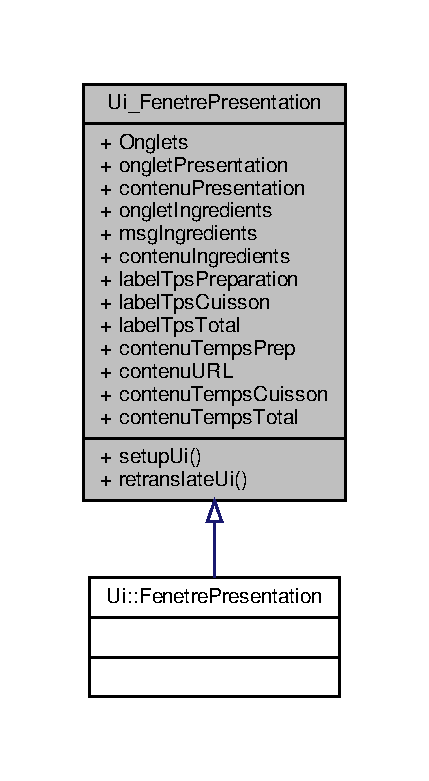
\includegraphics[width=200pt]{class_ui___fenetre_presentation__inherit__graph}
\end{center}
\end{figure}
\subsection*{Fonctions membres publiques}
\begin{DoxyCompactItemize}
\item 
void \hyperlink{class_ui___fenetre_presentation_a08e799fcf97f8afe980e76770b4ef960}{setup\+Ui} (Q\+Widget $\ast$Fenetre\+Presentation)
\item 
void \hyperlink{class_ui___fenetre_presentation_a14a00db87b3b4ce5a1e3df9f754e19bb}{retranslate\+Ui} (Q\+Widget $\ast$Fenetre\+Presentation)
\end{DoxyCompactItemize}
\subsection*{Attributs publics}
\begin{DoxyCompactItemize}
\item 
Q\+Tab\+Widget $\ast$ \hyperlink{class_ui___fenetre_presentation_a5ada401c3f50deda8794ad915e047707}{Onglets}
\item 
Q\+Widget $\ast$ \hyperlink{class_ui___fenetre_presentation_a6569025596a4f21aad52d42c4c0cde3d}{onglet\+Presentation}
\item 
Q\+List\+Widget $\ast$ \hyperlink{class_ui___fenetre_presentation_a15b1c966591fea35f2769207cfa21a0e}{contenu\+Presentation}
\item 
Q\+Widget $\ast$ \hyperlink{class_ui___fenetre_presentation_ade5aa5e1df3a3f800400499917077fb2}{onglet\+Ingredients}
\item 
Q\+Label $\ast$ \hyperlink{class_ui___fenetre_presentation_a6bd65740a513271b28bbd9e72f05df01}{msg\+Ingredients}
\item 
Q\+List\+Widget $\ast$ \hyperlink{class_ui___fenetre_presentation_a35b6dfdfa4899c487169582542e5b3e0}{contenu\+Ingredients}
\item 
Q\+Label $\ast$ \hyperlink{class_ui___fenetre_presentation_aa7aae419a87c0248c735670010e2a38a}{label\+Tps\+Preparation}
\item 
Q\+Label $\ast$ \hyperlink{class_ui___fenetre_presentation_ace7dcf1ffe9dbab894494f4b0bbdaa48}{label\+Tps\+Cuisson}
\item 
Q\+Label $\ast$ \hyperlink{class_ui___fenetre_presentation_a9bf87a50c0a4ee15739d7800c777614b}{label\+Tps\+Total}
\item 
Q\+List\+View $\ast$ \hyperlink{class_ui___fenetre_presentation_a90bdc54b6b901eb9aae58ef440bc8963}{contenu\+Temps\+Prep}
\item 
Q\+List\+View $\ast$ \hyperlink{class_ui___fenetre_presentation_ad266b41d115254cbe73186a30dee0d12}{contenu\+U\+RL}
\item 
Q\+List\+View $\ast$ \hyperlink{class_ui___fenetre_presentation_a3efaca6db5e151ffbd20f7cad1f94dfb}{contenu\+Temps\+Cuisson}
\item 
Q\+List\+View $\ast$ \hyperlink{class_ui___fenetre_presentation_a1665db8ec6e2cf652f7de55d0deac678}{contenu\+Temps\+Total}
\end{DoxyCompactItemize}


\subsection{Documentation des fonctions membres}
\mbox{\Hypertarget{class_ui___fenetre_presentation_a14a00db87b3b4ce5a1e3df9f754e19bb}\label{class_ui___fenetre_presentation_a14a00db87b3b4ce5a1e3df9f754e19bb}} 
\index{Ui\+\_\+\+Fenetre\+Presentation@{Ui\+\_\+\+Fenetre\+Presentation}!retranslate\+Ui@{retranslate\+Ui}}
\index{retranslate\+Ui@{retranslate\+Ui}!Ui\+\_\+\+Fenetre\+Presentation@{Ui\+\_\+\+Fenetre\+Presentation}}
\subsubsection{\texorpdfstring{retranslate\+Ui()}{retranslateUi()}}
{\footnotesize\ttfamily void Ui\+\_\+\+Fenetre\+Presentation\+::retranslate\+Ui (\begin{DoxyParamCaption}\item[{Q\+Widget $\ast$}]{Fenetre\+Presentation }\end{DoxyParamCaption})\hspace{0.3cm}{\ttfamily [inline]}}

\mbox{\Hypertarget{class_ui___fenetre_presentation_a08e799fcf97f8afe980e76770b4ef960}\label{class_ui___fenetre_presentation_a08e799fcf97f8afe980e76770b4ef960}} 
\index{Ui\+\_\+\+Fenetre\+Presentation@{Ui\+\_\+\+Fenetre\+Presentation}!setup\+Ui@{setup\+Ui}}
\index{setup\+Ui@{setup\+Ui}!Ui\+\_\+\+Fenetre\+Presentation@{Ui\+\_\+\+Fenetre\+Presentation}}
\subsubsection{\texorpdfstring{setup\+Ui()}{setupUi()}}
{\footnotesize\ttfamily void Ui\+\_\+\+Fenetre\+Presentation\+::setup\+Ui (\begin{DoxyParamCaption}\item[{Q\+Widget $\ast$}]{Fenetre\+Presentation }\end{DoxyParamCaption})\hspace{0.3cm}{\ttfamily [inline]}}



\subsection{Documentation des données membres}
\mbox{\Hypertarget{class_ui___fenetre_presentation_a35b6dfdfa4899c487169582542e5b3e0}\label{class_ui___fenetre_presentation_a35b6dfdfa4899c487169582542e5b3e0}} 
\index{Ui\+\_\+\+Fenetre\+Presentation@{Ui\+\_\+\+Fenetre\+Presentation}!contenu\+Ingredients@{contenu\+Ingredients}}
\index{contenu\+Ingredients@{contenu\+Ingredients}!Ui\+\_\+\+Fenetre\+Presentation@{Ui\+\_\+\+Fenetre\+Presentation}}
\subsubsection{\texorpdfstring{contenu\+Ingredients}{contenuIngredients}}
{\footnotesize\ttfamily Q\+List\+Widget$\ast$ Ui\+\_\+\+Fenetre\+Presentation\+::contenu\+Ingredients}

\mbox{\Hypertarget{class_ui___fenetre_presentation_a15b1c966591fea35f2769207cfa21a0e}\label{class_ui___fenetre_presentation_a15b1c966591fea35f2769207cfa21a0e}} 
\index{Ui\+\_\+\+Fenetre\+Presentation@{Ui\+\_\+\+Fenetre\+Presentation}!contenu\+Presentation@{contenu\+Presentation}}
\index{contenu\+Presentation@{contenu\+Presentation}!Ui\+\_\+\+Fenetre\+Presentation@{Ui\+\_\+\+Fenetre\+Presentation}}
\subsubsection{\texorpdfstring{contenu\+Presentation}{contenuPresentation}}
{\footnotesize\ttfamily Q\+List\+Widget$\ast$ Ui\+\_\+\+Fenetre\+Presentation\+::contenu\+Presentation}

\mbox{\Hypertarget{class_ui___fenetre_presentation_a3efaca6db5e151ffbd20f7cad1f94dfb}\label{class_ui___fenetre_presentation_a3efaca6db5e151ffbd20f7cad1f94dfb}} 
\index{Ui\+\_\+\+Fenetre\+Presentation@{Ui\+\_\+\+Fenetre\+Presentation}!contenu\+Temps\+Cuisson@{contenu\+Temps\+Cuisson}}
\index{contenu\+Temps\+Cuisson@{contenu\+Temps\+Cuisson}!Ui\+\_\+\+Fenetre\+Presentation@{Ui\+\_\+\+Fenetre\+Presentation}}
\subsubsection{\texorpdfstring{contenu\+Temps\+Cuisson}{contenuTempsCuisson}}
{\footnotesize\ttfamily Q\+List\+View$\ast$ Ui\+\_\+\+Fenetre\+Presentation\+::contenu\+Temps\+Cuisson}

\mbox{\Hypertarget{class_ui___fenetre_presentation_a90bdc54b6b901eb9aae58ef440bc8963}\label{class_ui___fenetre_presentation_a90bdc54b6b901eb9aae58ef440bc8963}} 
\index{Ui\+\_\+\+Fenetre\+Presentation@{Ui\+\_\+\+Fenetre\+Presentation}!contenu\+Temps\+Prep@{contenu\+Temps\+Prep}}
\index{contenu\+Temps\+Prep@{contenu\+Temps\+Prep}!Ui\+\_\+\+Fenetre\+Presentation@{Ui\+\_\+\+Fenetre\+Presentation}}
\subsubsection{\texorpdfstring{contenu\+Temps\+Prep}{contenuTempsPrep}}
{\footnotesize\ttfamily Q\+List\+View$\ast$ Ui\+\_\+\+Fenetre\+Presentation\+::contenu\+Temps\+Prep}

\mbox{\Hypertarget{class_ui___fenetre_presentation_a1665db8ec6e2cf652f7de55d0deac678}\label{class_ui___fenetre_presentation_a1665db8ec6e2cf652f7de55d0deac678}} 
\index{Ui\+\_\+\+Fenetre\+Presentation@{Ui\+\_\+\+Fenetre\+Presentation}!contenu\+Temps\+Total@{contenu\+Temps\+Total}}
\index{contenu\+Temps\+Total@{contenu\+Temps\+Total}!Ui\+\_\+\+Fenetre\+Presentation@{Ui\+\_\+\+Fenetre\+Presentation}}
\subsubsection{\texorpdfstring{contenu\+Temps\+Total}{contenuTempsTotal}}
{\footnotesize\ttfamily Q\+List\+View$\ast$ Ui\+\_\+\+Fenetre\+Presentation\+::contenu\+Temps\+Total}

\mbox{\Hypertarget{class_ui___fenetre_presentation_ad266b41d115254cbe73186a30dee0d12}\label{class_ui___fenetre_presentation_ad266b41d115254cbe73186a30dee0d12}} 
\index{Ui\+\_\+\+Fenetre\+Presentation@{Ui\+\_\+\+Fenetre\+Presentation}!contenu\+U\+RL@{contenu\+U\+RL}}
\index{contenu\+U\+RL@{contenu\+U\+RL}!Ui\+\_\+\+Fenetre\+Presentation@{Ui\+\_\+\+Fenetre\+Presentation}}
\subsubsection{\texorpdfstring{contenu\+U\+RL}{contenuURL}}
{\footnotesize\ttfamily Q\+List\+View$\ast$ Ui\+\_\+\+Fenetre\+Presentation\+::contenu\+U\+RL}

\mbox{\Hypertarget{class_ui___fenetre_presentation_ace7dcf1ffe9dbab894494f4b0bbdaa48}\label{class_ui___fenetre_presentation_ace7dcf1ffe9dbab894494f4b0bbdaa48}} 
\index{Ui\+\_\+\+Fenetre\+Presentation@{Ui\+\_\+\+Fenetre\+Presentation}!label\+Tps\+Cuisson@{label\+Tps\+Cuisson}}
\index{label\+Tps\+Cuisson@{label\+Tps\+Cuisson}!Ui\+\_\+\+Fenetre\+Presentation@{Ui\+\_\+\+Fenetre\+Presentation}}
\subsubsection{\texorpdfstring{label\+Tps\+Cuisson}{labelTpsCuisson}}
{\footnotesize\ttfamily Q\+Label$\ast$ Ui\+\_\+\+Fenetre\+Presentation\+::label\+Tps\+Cuisson}

\mbox{\Hypertarget{class_ui___fenetre_presentation_aa7aae419a87c0248c735670010e2a38a}\label{class_ui___fenetre_presentation_aa7aae419a87c0248c735670010e2a38a}} 
\index{Ui\+\_\+\+Fenetre\+Presentation@{Ui\+\_\+\+Fenetre\+Presentation}!label\+Tps\+Preparation@{label\+Tps\+Preparation}}
\index{label\+Tps\+Preparation@{label\+Tps\+Preparation}!Ui\+\_\+\+Fenetre\+Presentation@{Ui\+\_\+\+Fenetre\+Presentation}}
\subsubsection{\texorpdfstring{label\+Tps\+Preparation}{labelTpsPreparation}}
{\footnotesize\ttfamily Q\+Label$\ast$ Ui\+\_\+\+Fenetre\+Presentation\+::label\+Tps\+Preparation}

\mbox{\Hypertarget{class_ui___fenetre_presentation_a9bf87a50c0a4ee15739d7800c777614b}\label{class_ui___fenetre_presentation_a9bf87a50c0a4ee15739d7800c777614b}} 
\index{Ui\+\_\+\+Fenetre\+Presentation@{Ui\+\_\+\+Fenetre\+Presentation}!label\+Tps\+Total@{label\+Tps\+Total}}
\index{label\+Tps\+Total@{label\+Tps\+Total}!Ui\+\_\+\+Fenetre\+Presentation@{Ui\+\_\+\+Fenetre\+Presentation}}
\subsubsection{\texorpdfstring{label\+Tps\+Total}{labelTpsTotal}}
{\footnotesize\ttfamily Q\+Label$\ast$ Ui\+\_\+\+Fenetre\+Presentation\+::label\+Tps\+Total}

\mbox{\Hypertarget{class_ui___fenetre_presentation_a6bd65740a513271b28bbd9e72f05df01}\label{class_ui___fenetre_presentation_a6bd65740a513271b28bbd9e72f05df01}} 
\index{Ui\+\_\+\+Fenetre\+Presentation@{Ui\+\_\+\+Fenetre\+Presentation}!msg\+Ingredients@{msg\+Ingredients}}
\index{msg\+Ingredients@{msg\+Ingredients}!Ui\+\_\+\+Fenetre\+Presentation@{Ui\+\_\+\+Fenetre\+Presentation}}
\subsubsection{\texorpdfstring{msg\+Ingredients}{msgIngredients}}
{\footnotesize\ttfamily Q\+Label$\ast$ Ui\+\_\+\+Fenetre\+Presentation\+::msg\+Ingredients}

\mbox{\Hypertarget{class_ui___fenetre_presentation_ade5aa5e1df3a3f800400499917077fb2}\label{class_ui___fenetre_presentation_ade5aa5e1df3a3f800400499917077fb2}} 
\index{Ui\+\_\+\+Fenetre\+Presentation@{Ui\+\_\+\+Fenetre\+Presentation}!onglet\+Ingredients@{onglet\+Ingredients}}
\index{onglet\+Ingredients@{onglet\+Ingredients}!Ui\+\_\+\+Fenetre\+Presentation@{Ui\+\_\+\+Fenetre\+Presentation}}
\subsubsection{\texorpdfstring{onglet\+Ingredients}{ongletIngredients}}
{\footnotesize\ttfamily Q\+Widget$\ast$ Ui\+\_\+\+Fenetre\+Presentation\+::onglet\+Ingredients}

\mbox{\Hypertarget{class_ui___fenetre_presentation_a6569025596a4f21aad52d42c4c0cde3d}\label{class_ui___fenetre_presentation_a6569025596a4f21aad52d42c4c0cde3d}} 
\index{Ui\+\_\+\+Fenetre\+Presentation@{Ui\+\_\+\+Fenetre\+Presentation}!onglet\+Presentation@{onglet\+Presentation}}
\index{onglet\+Presentation@{onglet\+Presentation}!Ui\+\_\+\+Fenetre\+Presentation@{Ui\+\_\+\+Fenetre\+Presentation}}
\subsubsection{\texorpdfstring{onglet\+Presentation}{ongletPresentation}}
{\footnotesize\ttfamily Q\+Widget$\ast$ Ui\+\_\+\+Fenetre\+Presentation\+::onglet\+Presentation}

\mbox{\Hypertarget{class_ui___fenetre_presentation_a5ada401c3f50deda8794ad915e047707}\label{class_ui___fenetre_presentation_a5ada401c3f50deda8794ad915e047707}} 
\index{Ui\+\_\+\+Fenetre\+Presentation@{Ui\+\_\+\+Fenetre\+Presentation}!Onglets@{Onglets}}
\index{Onglets@{Onglets}!Ui\+\_\+\+Fenetre\+Presentation@{Ui\+\_\+\+Fenetre\+Presentation}}
\subsubsection{\texorpdfstring{Onglets}{Onglets}}
{\footnotesize\ttfamily Q\+Tab\+Widget$\ast$ Ui\+\_\+\+Fenetre\+Presentation\+::\+Onglets}



La documentation de cette classe a été générée à partir du fichier suivant \+:\begin{DoxyCompactItemize}
\item 
Lecteur\+Recette/\hyperlink{ui__presentation_8h}{ui\+\_\+presentation.\+h}\end{DoxyCompactItemize}

\hypertarget{class_ui___main_window}{}\section{Référence de la classe Ui\+\_\+\+Main\+Window}
\label{class_ui___main_window}\index{Ui\+\_\+\+Main\+Window@{Ui\+\_\+\+Main\+Window}}


{\ttfamily \#include $<$ui\+\_\+mainwindow.\+h$>$}



Graphe d\textquotesingle{}héritage de Ui\+\_\+\+Main\+Window\+:
\nopagebreak
\begin{figure}[H]
\begin{center}
\leavevmode
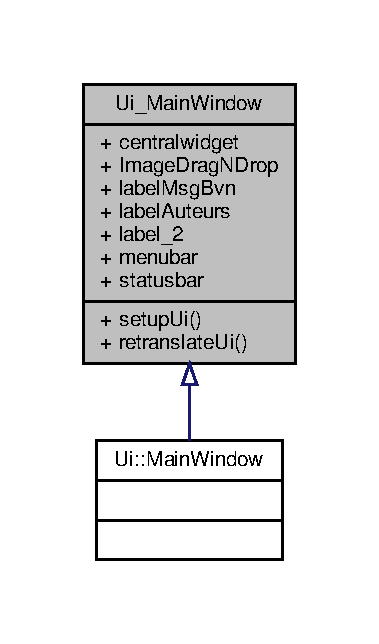
\includegraphics[width=182pt]{class_ui___main_window__inherit__graph}
\end{center}
\end{figure}


Graphe de collaboration de Ui\+\_\+\+Main\+Window\+:
\nopagebreak
\begin{figure}[H]
\begin{center}
\leavevmode
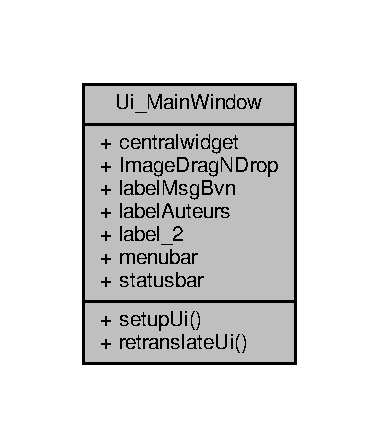
\includegraphics[width=182pt]{class_ui___main_window__coll__graph}
\end{center}
\end{figure}
\subsection*{Fonctions membres publiques}
\begin{DoxyCompactItemize}
\item 
void \hyperlink{class_ui___main_window_acf4a0872c4c77d8f43a2ec66ed849b58}{setup\+Ui} (Q\+Main\+Window $\ast$\hyperlink{class_main_window}{Main\+Window})
\item 
void \hyperlink{class_ui___main_window_a097dd160c3534a204904cb374412c618}{retranslate\+Ui} (Q\+Main\+Window $\ast$\hyperlink{class_main_window}{Main\+Window})
\end{DoxyCompactItemize}
\subsection*{Attributs publics}
\begin{DoxyCompactItemize}
\item 
Q\+Widget $\ast$ \hyperlink{class_ui___main_window_a356f1cf3ebda15f1fac59467ee081b74}{centralwidget}
\item 
Q\+Label $\ast$ \hyperlink{class_ui___main_window_ab0067ac42360f3cf2bb414b788d22f8e}{Image\+Drag\+N\+Drop}
\item 
Q\+Label $\ast$ \hyperlink{class_ui___main_window_a06205a0a8713b97da37a408c9dd3058e}{label\+Msg\+Bvn}
\item 
Q\+Label $\ast$ \hyperlink{class_ui___main_window_ae3a2caa0dbf4539a0bd06f4e35ddc537}{label\+Auteurs}
\item 
Q\+Label $\ast$ \hyperlink{class_ui___main_window_a2e2516d755e4dd53fc905dabddf2738a}{label\+\_\+2}
\item 
Q\+Menu\+Bar $\ast$ \hyperlink{class_ui___main_window_adf43d9a67adaec750aaa956b5e082f09}{menubar}
\item 
Q\+Status\+Bar $\ast$ \hyperlink{class_ui___main_window_a1687cceb1e2787aa1f83e50433943a91}{statusbar}
\end{DoxyCompactItemize}


\subsection{Documentation des fonctions membres}
\mbox{\Hypertarget{class_ui___main_window_a097dd160c3534a204904cb374412c618}\label{class_ui___main_window_a097dd160c3534a204904cb374412c618}} 
\index{Ui\+\_\+\+Main\+Window@{Ui\+\_\+\+Main\+Window}!retranslate\+Ui@{retranslate\+Ui}}
\index{retranslate\+Ui@{retranslate\+Ui}!Ui\+\_\+\+Main\+Window@{Ui\+\_\+\+Main\+Window}}
\subsubsection{\texorpdfstring{retranslate\+Ui()}{retranslateUi()}}
{\footnotesize\ttfamily void Ui\+\_\+\+Main\+Window\+::retranslate\+Ui (\begin{DoxyParamCaption}\item[{Q\+Main\+Window $\ast$}]{Main\+Window }\end{DoxyParamCaption})\hspace{0.3cm}{\ttfamily [inline]}}

Voici le graphe des appelants de cette fonction \+:
\nopagebreak
\begin{figure}[H]
\begin{center}
\leavevmode
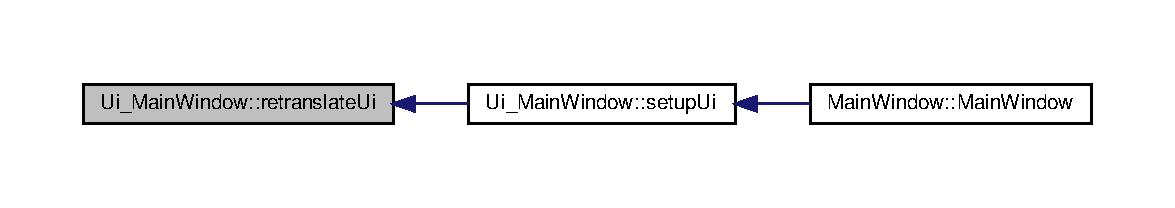
\includegraphics[width=350pt]{class_ui___main_window_a097dd160c3534a204904cb374412c618_icgraph}
\end{center}
\end{figure}
\mbox{\Hypertarget{class_ui___main_window_acf4a0872c4c77d8f43a2ec66ed849b58}\label{class_ui___main_window_acf4a0872c4c77d8f43a2ec66ed849b58}} 
\index{Ui\+\_\+\+Main\+Window@{Ui\+\_\+\+Main\+Window}!setup\+Ui@{setup\+Ui}}
\index{setup\+Ui@{setup\+Ui}!Ui\+\_\+\+Main\+Window@{Ui\+\_\+\+Main\+Window}}
\subsubsection{\texorpdfstring{setup\+Ui()}{setupUi()}}
{\footnotesize\ttfamily void Ui\+\_\+\+Main\+Window\+::setup\+Ui (\begin{DoxyParamCaption}\item[{Q\+Main\+Window $\ast$}]{Main\+Window }\end{DoxyParamCaption})\hspace{0.3cm}{\ttfamily [inline]}}

Voici le graphe d\textquotesingle{}appel pour cette fonction \+:
\nopagebreak
\begin{figure}[H]
\begin{center}
\leavevmode
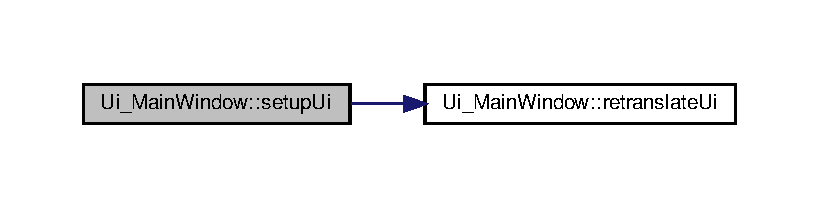
\includegraphics[width=350pt]{class_ui___main_window_acf4a0872c4c77d8f43a2ec66ed849b58_cgraph}
\end{center}
\end{figure}
Voici le graphe des appelants de cette fonction \+:
\nopagebreak
\begin{figure}[H]
\begin{center}
\leavevmode
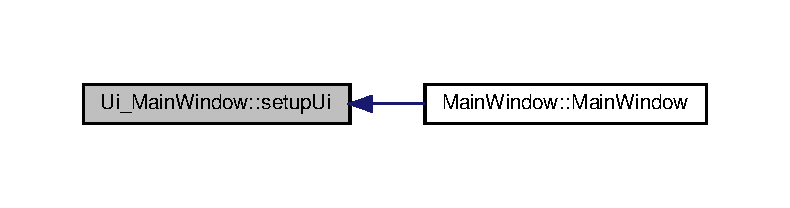
\includegraphics[width=350pt]{class_ui___main_window_acf4a0872c4c77d8f43a2ec66ed849b58_icgraph}
\end{center}
\end{figure}


\subsection{Documentation des données membres}
\mbox{\Hypertarget{class_ui___main_window_a356f1cf3ebda15f1fac59467ee081b74}\label{class_ui___main_window_a356f1cf3ebda15f1fac59467ee081b74}} 
\index{Ui\+\_\+\+Main\+Window@{Ui\+\_\+\+Main\+Window}!centralwidget@{centralwidget}}
\index{centralwidget@{centralwidget}!Ui\+\_\+\+Main\+Window@{Ui\+\_\+\+Main\+Window}}
\subsubsection{\texorpdfstring{centralwidget}{centralwidget}}
{\footnotesize\ttfamily Q\+Widget$\ast$ Ui\+\_\+\+Main\+Window\+::centralwidget}

\mbox{\Hypertarget{class_ui___main_window_ab0067ac42360f3cf2bb414b788d22f8e}\label{class_ui___main_window_ab0067ac42360f3cf2bb414b788d22f8e}} 
\index{Ui\+\_\+\+Main\+Window@{Ui\+\_\+\+Main\+Window}!Image\+Drag\+N\+Drop@{Image\+Drag\+N\+Drop}}
\index{Image\+Drag\+N\+Drop@{Image\+Drag\+N\+Drop}!Ui\+\_\+\+Main\+Window@{Ui\+\_\+\+Main\+Window}}
\subsubsection{\texorpdfstring{Image\+Drag\+N\+Drop}{ImageDragNDrop}}
{\footnotesize\ttfamily Q\+Label$\ast$ Ui\+\_\+\+Main\+Window\+::\+Image\+Drag\+N\+Drop}

\mbox{\Hypertarget{class_ui___main_window_a2e2516d755e4dd53fc905dabddf2738a}\label{class_ui___main_window_a2e2516d755e4dd53fc905dabddf2738a}} 
\index{Ui\+\_\+\+Main\+Window@{Ui\+\_\+\+Main\+Window}!label\+\_\+2@{label\+\_\+2}}
\index{label\+\_\+2@{label\+\_\+2}!Ui\+\_\+\+Main\+Window@{Ui\+\_\+\+Main\+Window}}
\subsubsection{\texorpdfstring{label\+\_\+2}{label\_2}}
{\footnotesize\ttfamily Q\+Label$\ast$ Ui\+\_\+\+Main\+Window\+::label\+\_\+2}

\mbox{\Hypertarget{class_ui___main_window_ae3a2caa0dbf4539a0bd06f4e35ddc537}\label{class_ui___main_window_ae3a2caa0dbf4539a0bd06f4e35ddc537}} 
\index{Ui\+\_\+\+Main\+Window@{Ui\+\_\+\+Main\+Window}!label\+Auteurs@{label\+Auteurs}}
\index{label\+Auteurs@{label\+Auteurs}!Ui\+\_\+\+Main\+Window@{Ui\+\_\+\+Main\+Window}}
\subsubsection{\texorpdfstring{label\+Auteurs}{labelAuteurs}}
{\footnotesize\ttfamily Q\+Label$\ast$ Ui\+\_\+\+Main\+Window\+::label\+Auteurs}

\mbox{\Hypertarget{class_ui___main_window_a06205a0a8713b97da37a408c9dd3058e}\label{class_ui___main_window_a06205a0a8713b97da37a408c9dd3058e}} 
\index{Ui\+\_\+\+Main\+Window@{Ui\+\_\+\+Main\+Window}!label\+Msg\+Bvn@{label\+Msg\+Bvn}}
\index{label\+Msg\+Bvn@{label\+Msg\+Bvn}!Ui\+\_\+\+Main\+Window@{Ui\+\_\+\+Main\+Window}}
\subsubsection{\texorpdfstring{label\+Msg\+Bvn}{labelMsgBvn}}
{\footnotesize\ttfamily Q\+Label$\ast$ Ui\+\_\+\+Main\+Window\+::label\+Msg\+Bvn}

\mbox{\Hypertarget{class_ui___main_window_adf43d9a67adaec750aaa956b5e082f09}\label{class_ui___main_window_adf43d9a67adaec750aaa956b5e082f09}} 
\index{Ui\+\_\+\+Main\+Window@{Ui\+\_\+\+Main\+Window}!menubar@{menubar}}
\index{menubar@{menubar}!Ui\+\_\+\+Main\+Window@{Ui\+\_\+\+Main\+Window}}
\subsubsection{\texorpdfstring{menubar}{menubar}}
{\footnotesize\ttfamily Q\+Menu\+Bar$\ast$ Ui\+\_\+\+Main\+Window\+::menubar}

\mbox{\Hypertarget{class_ui___main_window_a1687cceb1e2787aa1f83e50433943a91}\label{class_ui___main_window_a1687cceb1e2787aa1f83e50433943a91}} 
\index{Ui\+\_\+\+Main\+Window@{Ui\+\_\+\+Main\+Window}!statusbar@{statusbar}}
\index{statusbar@{statusbar}!Ui\+\_\+\+Main\+Window@{Ui\+\_\+\+Main\+Window}}
\subsubsection{\texorpdfstring{statusbar}{statusbar}}
{\footnotesize\ttfamily Q\+Status\+Bar$\ast$ Ui\+\_\+\+Main\+Window\+::statusbar}



La documentation de cette classe a été générée à partir du fichier suivant \+:\begin{DoxyCompactItemize}
\item 
Lecteur\+Recette/\hyperlink{ui__mainwindow_8h}{ui\+\_\+mainwindow.\+h}\end{DoxyCompactItemize}

\chapter{Documentation des fichiers}
\hypertarget{_lecteur_json_8cpp}{}\section{Référence du fichier Lecteur\+Recette/\+Lecteur\+Json.cpp}
\label{_lecteur_json_8cpp}\index{Lecteur\+Recette/\+Lecteur\+Json.\+cpp@{Lecteur\+Recette/\+Lecteur\+Json.\+cpp}}


Programme qui lit le fichier J\+S\+ON et qui récupère les données.  


{\ttfamily \#include \char`\"{}lecteurjson.\+h\char`\"{}}\newline
Graphe des dépendances par inclusion de Lecteur\+Json.\+cpp\+:
\nopagebreak
\begin{figure}[H]
\begin{center}
\leavevmode
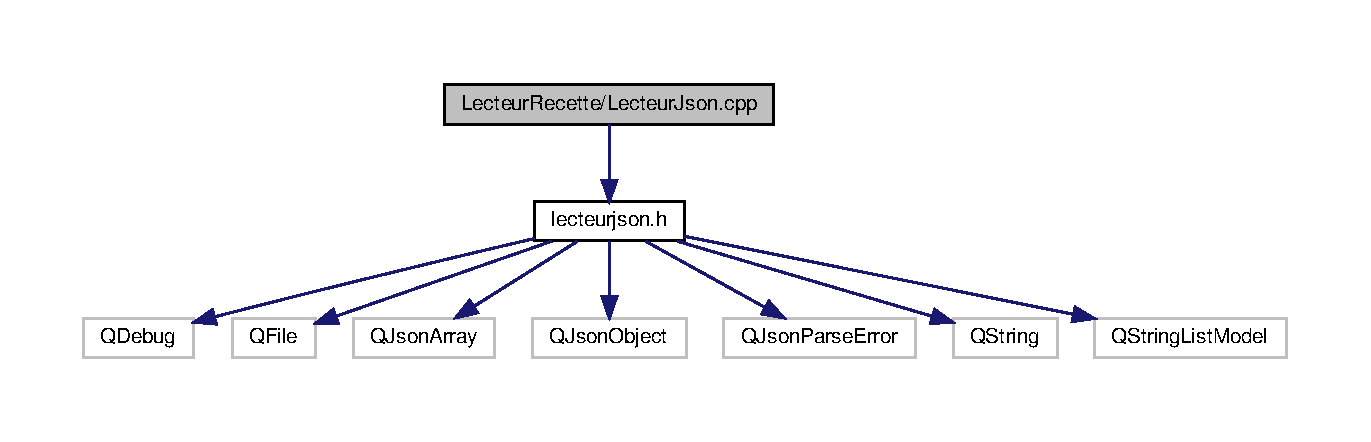
\includegraphics[width=350pt]{_lecteur_json_8cpp__incl}
\end{center}
\end{figure}


\subsection{Description détaillée}
Programme qui lit le fichier J\+S\+ON et qui récupère les données. 

\begin{DoxyAuthor}{Auteur}
Munoz Matteo -\/ Dufour Mattéo 
\end{DoxyAuthor}

\hypertarget{lecteurjson_8h}{}\section{Référence du fichier Lecteur\+Recette/lecteurjson.h}
\label{lecteurjson_8h}\index{Lecteur\+Recette/lecteurjson.\+h@{Lecteur\+Recette/lecteurjson.\+h}}


Récupération des éléments souhaiter dans le J\+S\+ON.  


{\ttfamily \#include $<$Q\+Debug$>$}\newline
{\ttfamily \#include $<$Q\+File$>$}\newline
{\ttfamily \#include $<$Q\+Json\+Array$>$}\newline
{\ttfamily \#include $<$Q\+Json\+Object$>$}\newline
{\ttfamily \#include $<$Q\+Json\+Parse\+Error$>$}\newline
{\ttfamily \#include $<$Q\+String$>$}\newline
{\ttfamily \#include $<$Q\+String\+List\+Model$>$}\newline
Graphe des dépendances par inclusion de lecteurjson.\+h\+:
\nopagebreak
\begin{figure}[H]
\begin{center}
\leavevmode
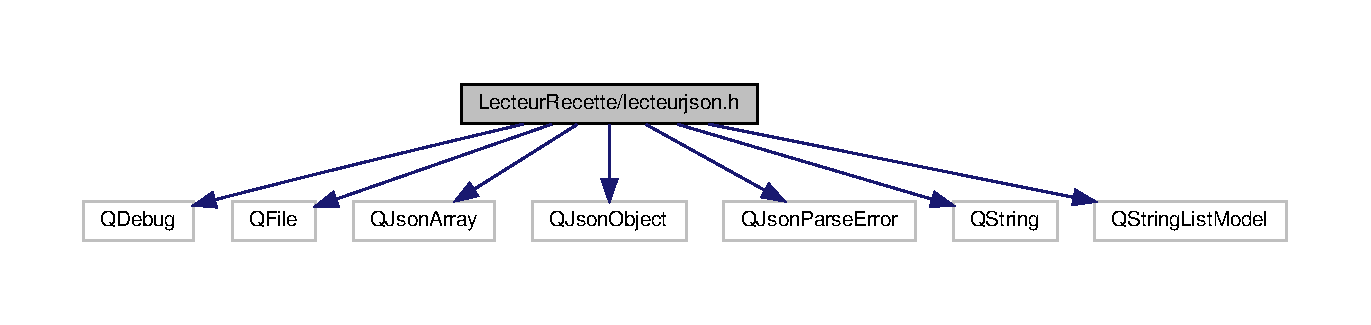
\includegraphics[width=350pt]{lecteurjson_8h__incl}
\end{center}
\end{figure}
Ce graphe montre quels fichiers incluent directement ou indirectement ce fichier \+:
\nopagebreak
\begin{figure}[H]
\begin{center}
\leavevmode
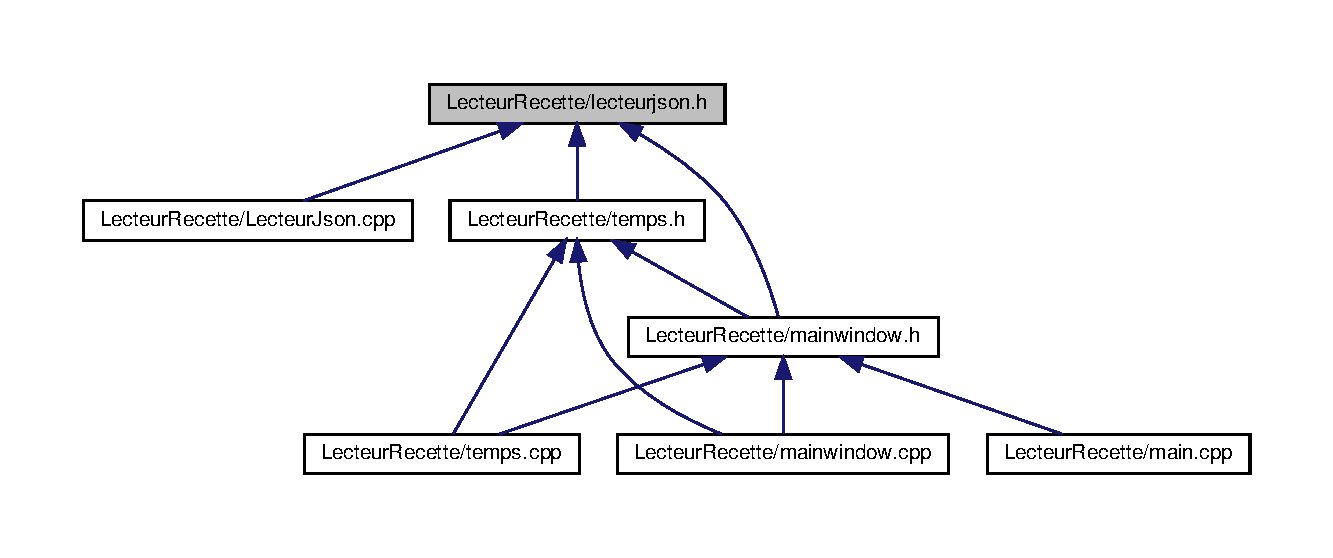
\includegraphics[width=350pt]{lecteurjson_8h__dep__incl}
\end{center}
\end{figure}
\subsection*{Classes}
\begin{DoxyCompactItemize}
\item 
class \hyperlink{class_lecteur_json}{Lecteur\+Json}
\begin{DoxyCompactList}\small\item\em Classe qui permet la lecture d\textquotesingle{}un fichier J\+S\+ON. \end{DoxyCompactList}\end{DoxyCompactItemize}


\subsection{Description détaillée}
Récupération des éléments souhaiter dans le J\+S\+ON. 

\begin{DoxyAuthor}{Auteur}
Munoz Matteo -\/ Dufour Mattéo 
\end{DoxyAuthor}

\hypertarget{main_8cpp}{}\section{Référence du fichier Lecteur\+Recette/main.cpp}
\label{main_8cpp}\index{Lecteur\+Recette/main.\+cpp@{Lecteur\+Recette/main.\+cpp}}


Programme principal.  


{\ttfamily \#include \char`\"{}mainwindow.\+h\char`\"{}}\newline
{\ttfamily \#include $<$Q\+Application$>$}\newline
Graphe des dépendances par inclusion de main.\+cpp\+:
\nopagebreak
\begin{figure}[H]
\begin{center}
\leavevmode
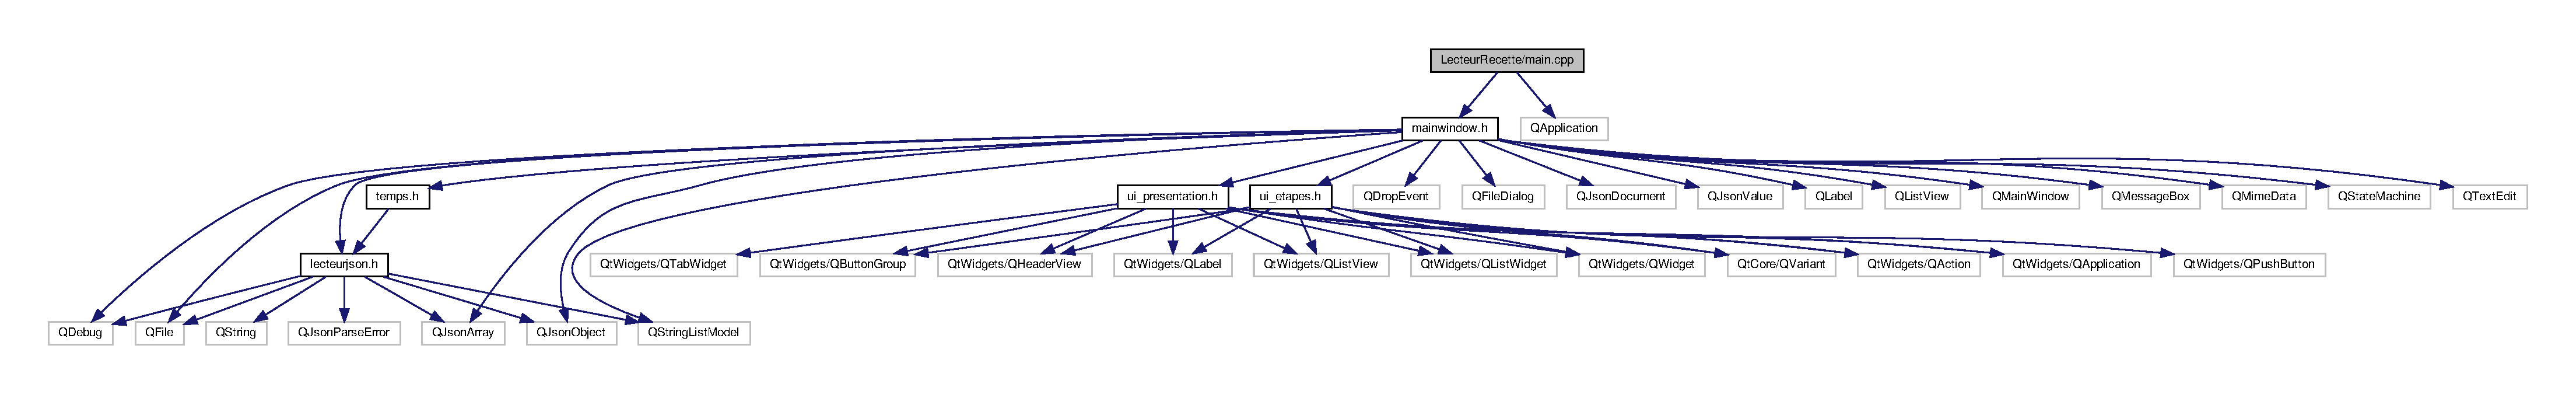
\includegraphics[width=350pt]{main_8cpp__incl}
\end{center}
\end{figure}
\subsection*{Fonctions}
\begin{DoxyCompactItemize}
\item 
int \hyperlink{main_8cpp_a0ddf1224851353fc92bfbff6f499fa97}{main} (int argc, char $\ast$argv\mbox{[}$\,$\mbox{]})
\end{DoxyCompactItemize}


\subsection{Description détaillée}
Programme principal. 

\begin{DoxyAuthor}{Auteur}
Munoz Matteo -\/ Dufour Mattéo 
\end{DoxyAuthor}


\subsection{Documentation des fonctions}
\mbox{\Hypertarget{main_8cpp_a0ddf1224851353fc92bfbff6f499fa97}\label{main_8cpp_a0ddf1224851353fc92bfbff6f499fa97}} 
\index{main.\+cpp@{main.\+cpp}!main@{main}}
\index{main@{main}!main.\+cpp@{main.\+cpp}}
\subsubsection{\texorpdfstring{main()}{main()}}
{\footnotesize\ttfamily int main (\begin{DoxyParamCaption}\item[{int}]{argc,  }\item[{char $\ast$}]{argv\mbox{[}$\,$\mbox{]} }\end{DoxyParamCaption})}


\hypertarget{mainwindow_8cpp}{}\section{Référence du fichier Lecteur\+Recette/mainwindow.cpp}
\label{mainwindow_8cpp}\index{Lecteur\+Recette/mainwindow.\+cpp@{Lecteur\+Recette/mainwindow.\+cpp}}


Programme qui gère tout l\textquotesingle{}affichage.  


{\ttfamily \#include \char`\"{}mainwindow.\+h\char`\"{}}\newline
{\ttfamily \#include \char`\"{}temps.\+h\char`\"{}}\newline
{\ttfamily \#include \char`\"{}ui\+\_\+mainwindow.\+h\char`\"{}}\newline
{\ttfamily \#include $<$Qt\+Debug$>$}\newline
Graphe des dépendances par inclusion de mainwindow.\+cpp\+:
\nopagebreak
\begin{figure}[H]
\begin{center}
\leavevmode
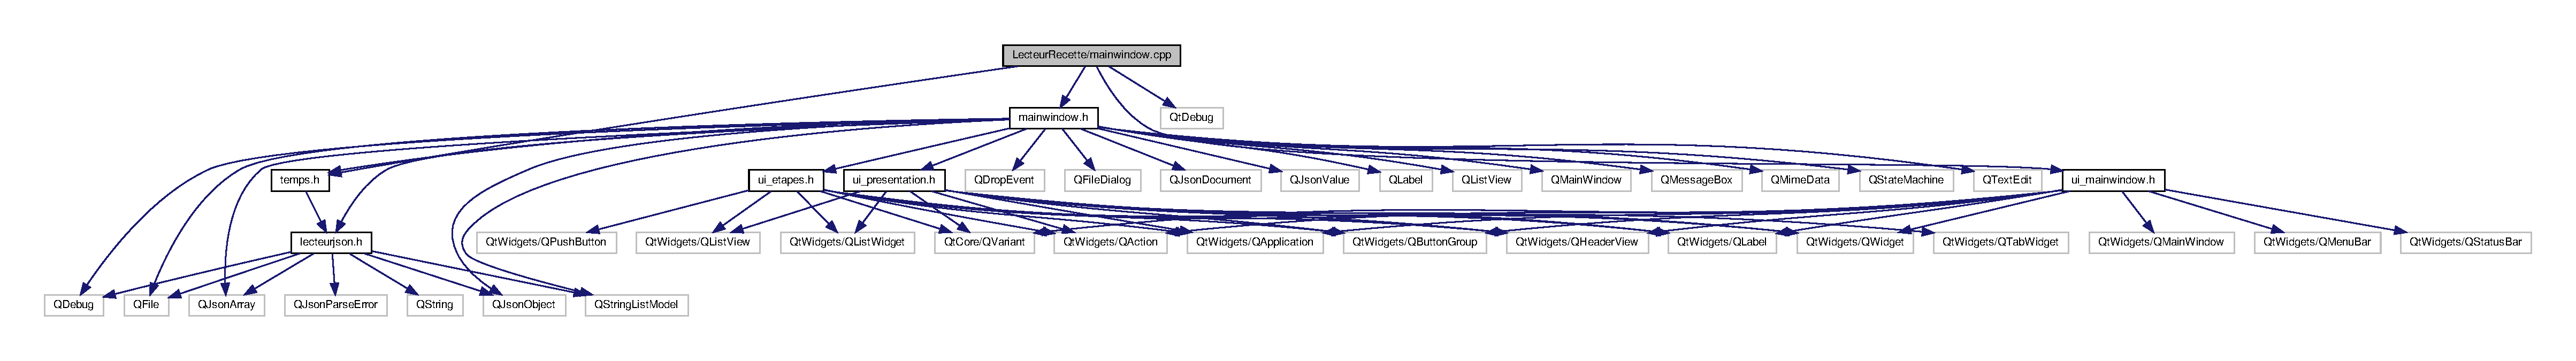
\includegraphics[width=350pt]{mainwindow_8cpp__incl}
\end{center}
\end{figure}


\subsection{Description détaillée}
Programme qui gère tout l\textquotesingle{}affichage. 

\begin{DoxyAuthor}{Auteur}
Munoz Matteo -\/ Dufour Mattéo 
\end{DoxyAuthor}

\hypertarget{mainwindow_8h}{}\section{mainwindow.\+h File Reference}
\label{mainwindow_8h}\index{mainwindow.\+h@{mainwindow.\+h}}


Classe des différentes fenêtre.  


{\ttfamily \#include \char`\"{}lecteurjson.\+h\char`\"{}}\newline
{\ttfamily \#include \char`\"{}temps.\+h\char`\"{}}\newline
{\ttfamily \#include \char`\"{}ui\+\_\+etapes.\+h\char`\"{}}\newline
{\ttfamily \#include \char`\"{}ui\+\_\+presentation.\+h\char`\"{}}\newline
{\ttfamily \#include $<$Q\+Debug$>$}\newline
{\ttfamily \#include $<$Q\+Drop\+Event$>$}\newline
{\ttfamily \#include $<$Q\+File$>$}\newline
{\ttfamily \#include $<$Q\+File\+Dialog$>$}\newline
{\ttfamily \#include $<$Q\+Json\+Array$>$}\newline
{\ttfamily \#include $<$Q\+Json\+Document$>$}\newline
{\ttfamily \#include $<$Q\+Json\+Object$>$}\newline
{\ttfamily \#include $<$Q\+Json\+Value$>$}\newline
{\ttfamily \#include $<$Q\+Label$>$}\newline
{\ttfamily \#include $<$Q\+List\+View$>$}\newline
{\ttfamily \#include $<$Q\+Main\+Window$>$}\newline
{\ttfamily \#include $<$Q\+Message\+Box$>$}\newline
{\ttfamily \#include $<$Q\+Mime\+Data$>$}\newline
{\ttfamily \#include $<$Q\+State\+Machine$>$}\newline
{\ttfamily \#include $<$Q\+String\+List\+Model$>$}\newline
{\ttfamily \#include $<$Q\+Text\+Edit$>$}\newline
Include dependency graph for mainwindow.\+h\+:
\nopagebreak
\begin{figure}[H]
\begin{center}
\leavevmode
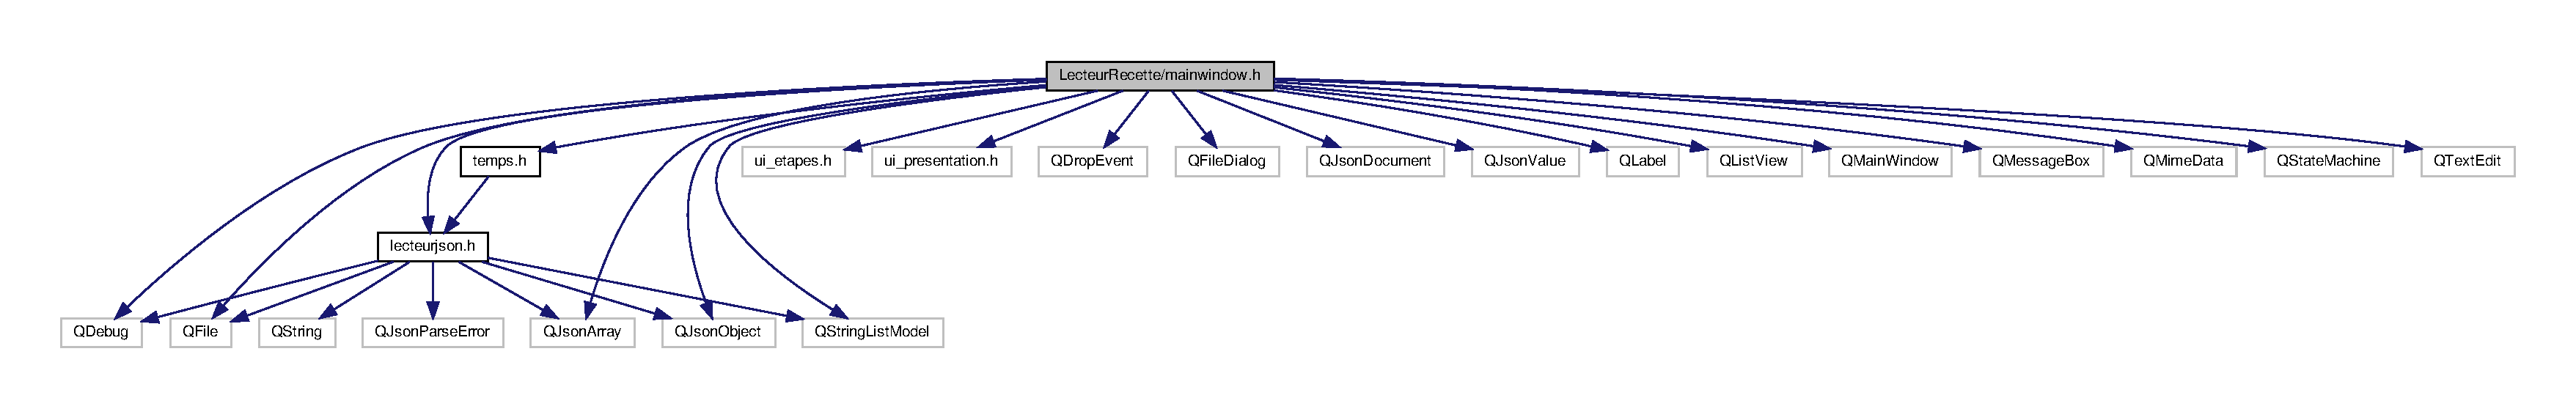
\includegraphics[width=350pt]{mainwindow_8h__incl}
\end{center}
\end{figure}
This graph shows which files directly or indirectly include this file\+:
\nopagebreak
\begin{figure}[H]
\begin{center}
\leavevmode
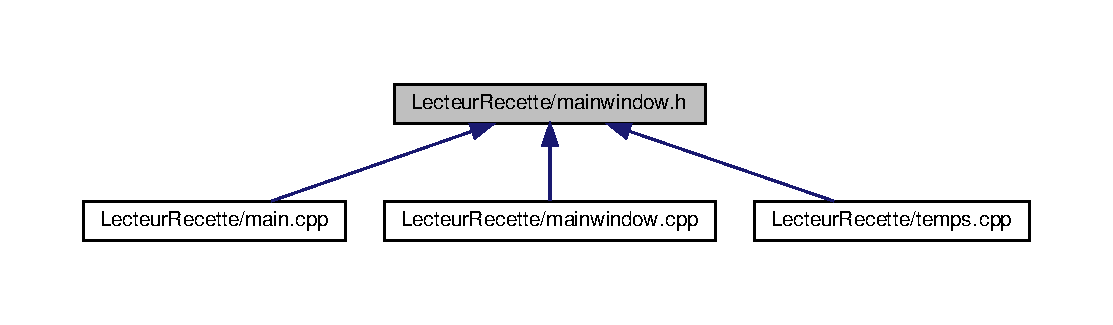
\includegraphics[width=323pt]{mainwindow_8h__dep__incl}
\end{center}
\end{figure}
\subsection*{Classes}
\begin{DoxyCompactItemize}
\item 
class \hyperlink{class_main_window}{Main\+Window}
\begin{DoxyCompactList}\small\item\em classe qui gère l\textquotesingle{}affichage des différentes fenêtres \end{DoxyCompactList}\end{DoxyCompactItemize}
\subsection*{Namespaces}
\begin{DoxyCompactItemize}
\item 
 \hyperlink{namespace_ui}{Ui}
\end{DoxyCompactItemize}


\subsection{Detailed Description}
Classe des différentes fenêtre. 

\begin{DoxyAuthor}{Author}
Munoz Matteo -\/ Dufour Mattéo 
\end{DoxyAuthor}

\hypertarget{temps_8cpp}{}\section{temps.\+cpp File Reference}
\label{temps_8cpp}\index{temps.\+cpp@{temps.\+cpp}}


Programme qui s\textquotesingle{}occupe du traitement du temps.  


{\ttfamily \#include \char`\"{}temps.\+h\char`\"{}}\newline
{\ttfamily \#include \char`\"{}mainwindow.\+h\char`\"{}}\newline
Include dependency graph for temps.\+cpp\+:
\nopagebreak
\begin{figure}[H]
\begin{center}
\leavevmode
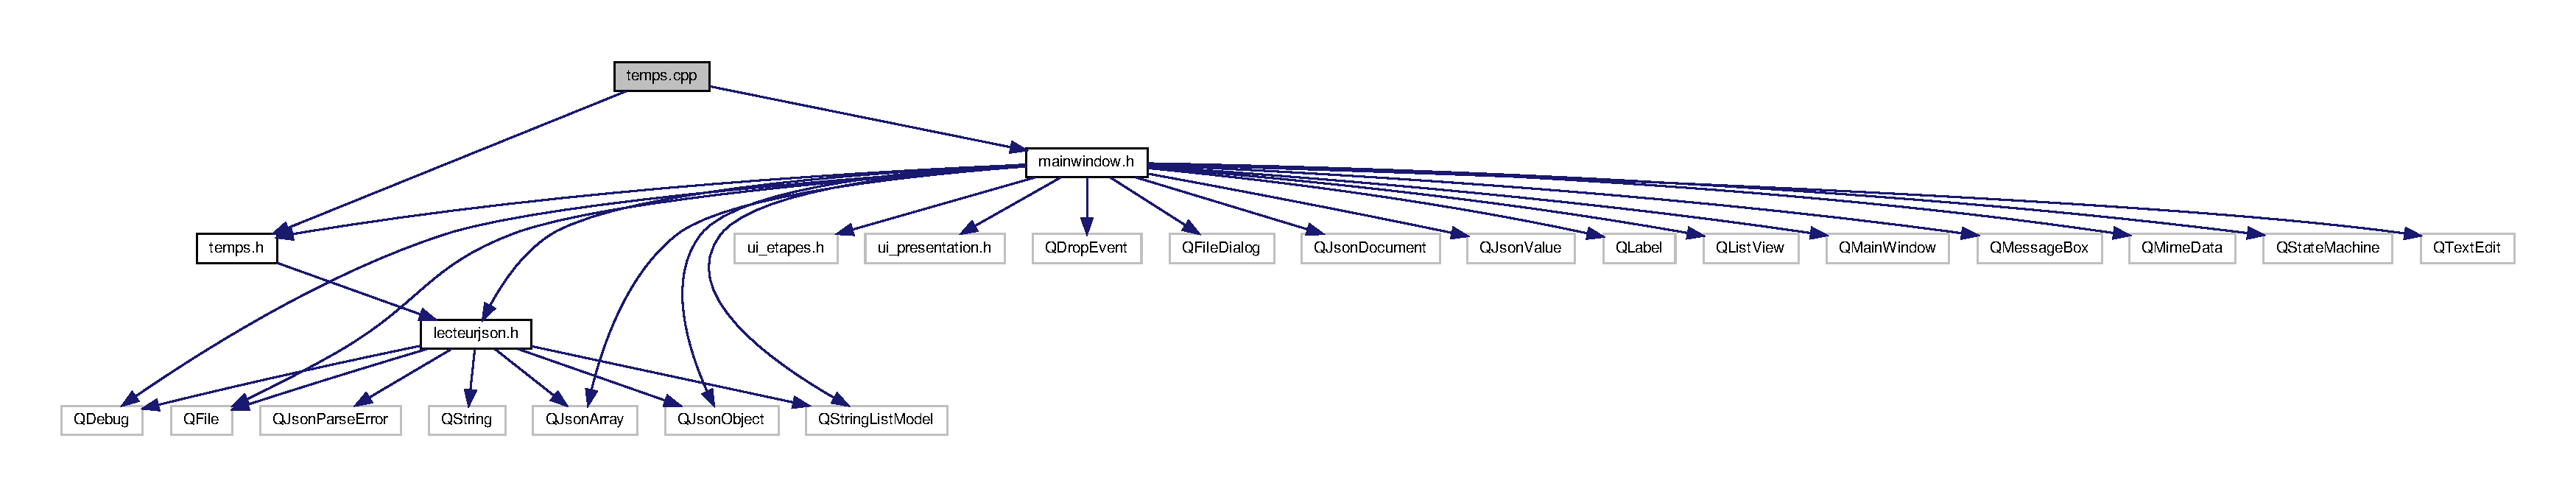
\includegraphics[width=350pt]{temps_8cpp__incl}
\end{center}
\end{figure}


\subsection{Detailed Description}
Programme qui s\textquotesingle{}occupe du traitement du temps. 

\begin{DoxyAuthor}{Author}
Munoz Matteo -\/ Dufour Mattéo 
\end{DoxyAuthor}

\hypertarget{temps_8h}{}\section{Référence du fichier Lecteur\+Recette/temps.h}
\label{temps_8h}\index{Lecteur\+Recette/temps.\+h@{Lecteur\+Recette/temps.\+h}}


Traitement donnée du programme.  


{\ttfamily \#include \char`\"{}lecteurjson.\+h\char`\"{}}\newline
Graphe des dépendances par inclusion de temps.\+h\+:
\nopagebreak
\begin{figure}[H]
\begin{center}
\leavevmode
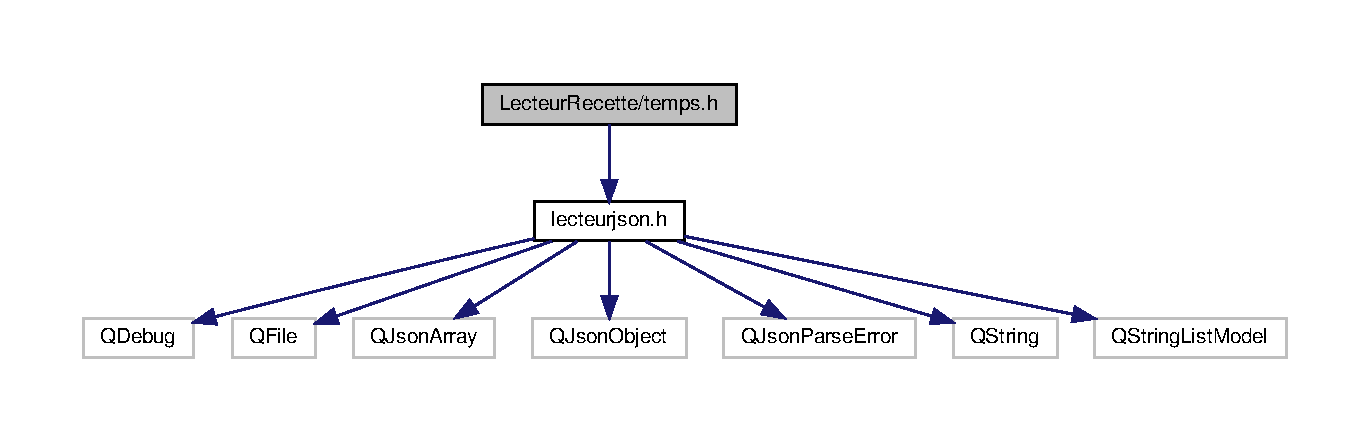
\includegraphics[width=350pt]{temps_8h__incl}
\end{center}
\end{figure}
Ce graphe montre quels fichiers incluent directement ou indirectement ce fichier \+:
\nopagebreak
\begin{figure}[H]
\begin{center}
\leavevmode
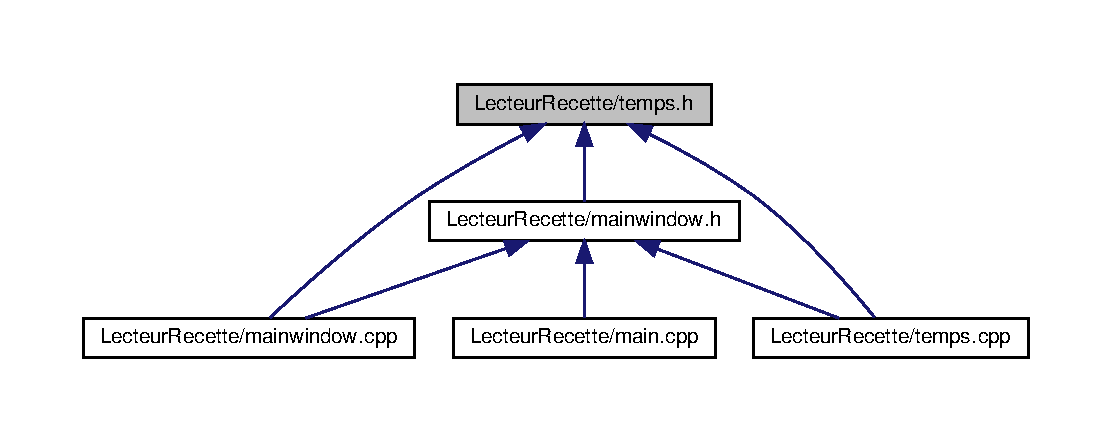
\includegraphics[width=350pt]{temps_8h__dep__incl}
\end{center}
\end{figure}
\subsection*{Classes}
\begin{DoxyCompactItemize}
\item 
class \hyperlink{classtraitement}{traitement}
\begin{DoxyCompactList}\small\item\em classe permettant le traitement du temps du fichier J\+Son \end{DoxyCompactList}\end{DoxyCompactItemize}


\subsection{Description détaillée}
Traitement donnée du programme. 

\begin{DoxyAuthor}{Auteur}
Munoz Matteo -\/ Dufour Mattéo 
\end{DoxyAuthor}

\hypertarget{ui__etapes_8h}{}\section{Référence du fichier Lecteur\+Recette/ui\+\_\+etapes.h}
\label{ui__etapes_8h}\index{Lecteur\+Recette/ui\+\_\+etapes.\+h@{Lecteur\+Recette/ui\+\_\+etapes.\+h}}
{\ttfamily \#include $<$Qt\+Core/\+Q\+Variant$>$}\newline
{\ttfamily \#include $<$Qt\+Widgets/\+Q\+Action$>$}\newline
{\ttfamily \#include $<$Qt\+Widgets/\+Q\+Application$>$}\newline
{\ttfamily \#include $<$Qt\+Widgets/\+Q\+Button\+Group$>$}\newline
{\ttfamily \#include $<$Qt\+Widgets/\+Q\+Header\+View$>$}\newline
{\ttfamily \#include $<$Qt\+Widgets/\+Q\+Label$>$}\newline
{\ttfamily \#include $<$Qt\+Widgets/\+Q\+List\+View$>$}\newline
{\ttfamily \#include $<$Qt\+Widgets/\+Q\+List\+Widget$>$}\newline
{\ttfamily \#include $<$Qt\+Widgets/\+Q\+Push\+Button$>$}\newline
{\ttfamily \#include $<$Qt\+Widgets/\+Q\+Widget$>$}\newline
Graphe des dépendances par inclusion de ui\+\_\+etapes.\+h\+:
\nopagebreak
\begin{figure}[H]
\begin{center}
\leavevmode
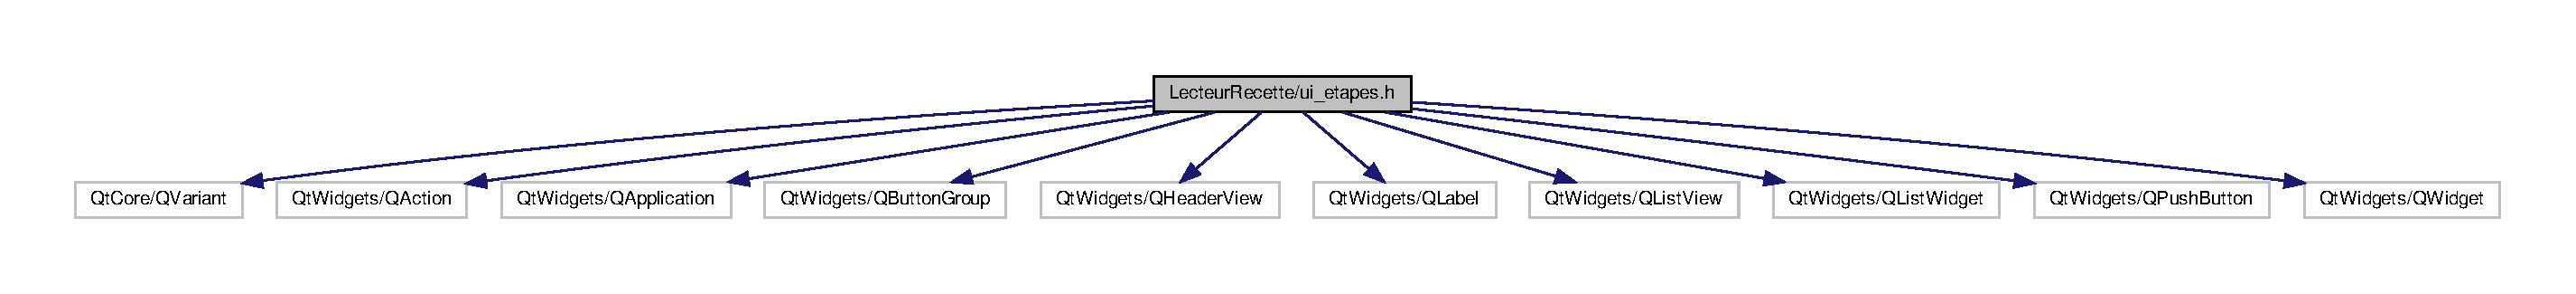
\includegraphics[width=350pt]{ui__etapes_8h__incl}
\end{center}
\end{figure}
Ce graphe montre quels fichiers incluent directement ou indirectement ce fichier \+:
\nopagebreak
\begin{figure}[H]
\begin{center}
\leavevmode
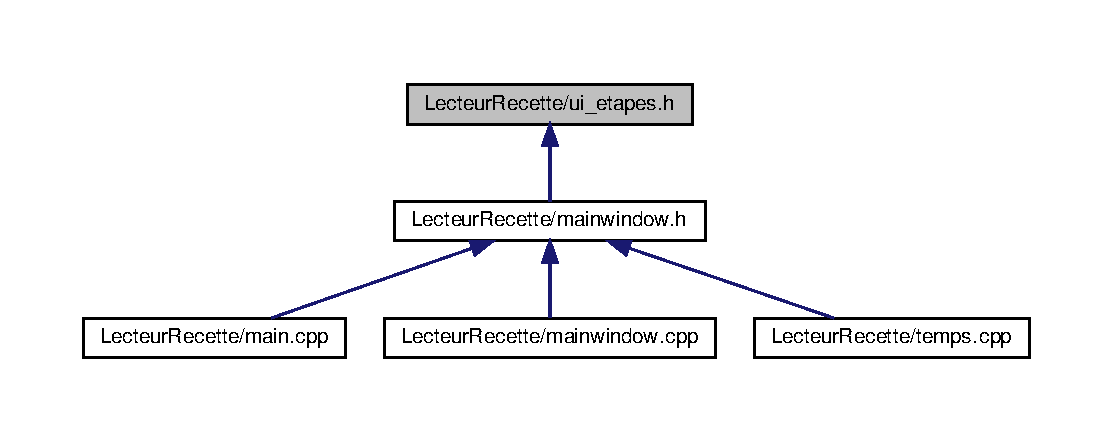
\includegraphics[width=350pt]{ui__etapes_8h__dep__incl}
\end{center}
\end{figure}
\subsection*{Classes}
\begin{DoxyCompactItemize}
\item 
class \hyperlink{class_ui___fenetre_etapes}{Ui\+\_\+\+Fenetre\+Etapes}
\item 
class \hyperlink{class_ui_1_1_fenetre_etapes}{Ui\+::\+Fenetre\+Etapes}
\end{DoxyCompactItemize}
\subsection*{Espaces de nommage}
\begin{DoxyCompactItemize}
\item 
 \hyperlink{namespace_ui}{Ui}
\end{DoxyCompactItemize}

\hypertarget{ui__mainwindow_8h}{}\section{Référence du fichier Lecteur\+Recette/ui\+\_\+mainwindow.h}
\label{ui__mainwindow_8h}\index{Lecteur\+Recette/ui\+\_\+mainwindow.\+h@{Lecteur\+Recette/ui\+\_\+mainwindow.\+h}}
{\ttfamily \#include $<$Qt\+Core/\+Q\+Variant$>$}\newline
{\ttfamily \#include $<$Qt\+Widgets/\+Q\+Action$>$}\newline
{\ttfamily \#include $<$Qt\+Widgets/\+Q\+Application$>$}\newline
{\ttfamily \#include $<$Qt\+Widgets/\+Q\+Button\+Group$>$}\newline
{\ttfamily \#include $<$Qt\+Widgets/\+Q\+Header\+View$>$}\newline
{\ttfamily \#include $<$Qt\+Widgets/\+Q\+Label$>$}\newline
{\ttfamily \#include $<$Qt\+Widgets/\+Q\+Main\+Window$>$}\newline
{\ttfamily \#include $<$Qt\+Widgets/\+Q\+Menu\+Bar$>$}\newline
{\ttfamily \#include $<$Qt\+Widgets/\+Q\+Status\+Bar$>$}\newline
{\ttfamily \#include $<$Qt\+Widgets/\+Q\+Widget$>$}\newline
Graphe des dépendances par inclusion de ui\+\_\+mainwindow.\+h\+:
\nopagebreak
\begin{figure}[H]
\begin{center}
\leavevmode
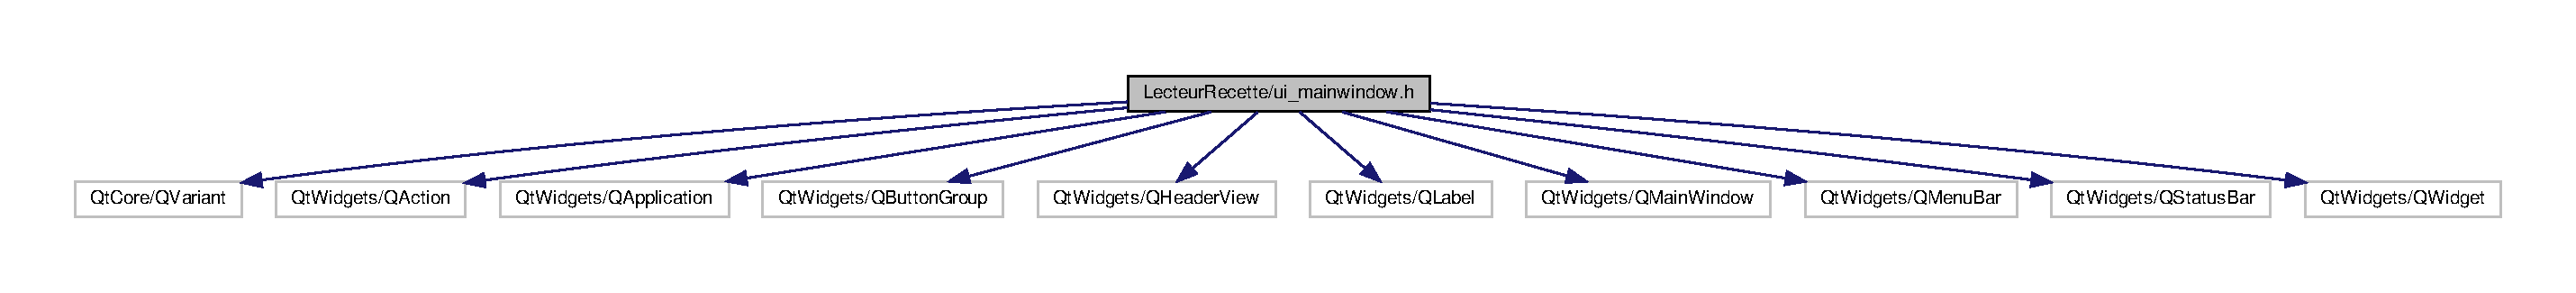
\includegraphics[width=350pt]{ui__mainwindow_8h__incl}
\end{center}
\end{figure}
Ce graphe montre quels fichiers incluent directement ou indirectement ce fichier \+:
\nopagebreak
\begin{figure}[H]
\begin{center}
\leavevmode
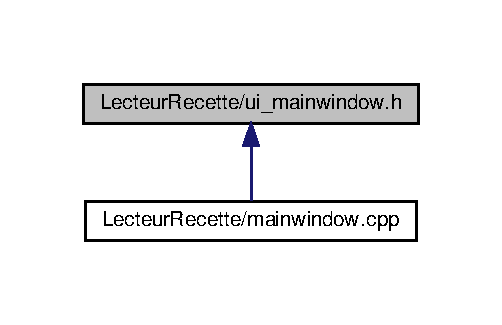
\includegraphics[width=241pt]{ui__mainwindow_8h__dep__incl}
\end{center}
\end{figure}
\subsection*{Classes}
\begin{DoxyCompactItemize}
\item 
class \hyperlink{class_ui___main_window}{Ui\+\_\+\+Main\+Window}
\item 
class \hyperlink{class_ui_1_1_main_window}{Ui\+::\+Main\+Window}
\end{DoxyCompactItemize}
\subsection*{Espaces de nommage}
\begin{DoxyCompactItemize}
\item 
 \hyperlink{namespace_ui}{Ui}
\end{DoxyCompactItemize}

\hypertarget{ui__presentation_8h}{}\section{Référence du fichier Lecteur\+Recette/ui\+\_\+presentation.h}
\label{ui__presentation_8h}\index{Lecteur\+Recette/ui\+\_\+presentation.\+h@{Lecteur\+Recette/ui\+\_\+presentation.\+h}}
{\ttfamily \#include $<$Qt\+Core/\+Q\+Variant$>$}\newline
{\ttfamily \#include $<$Qt\+Widgets/\+Q\+Action$>$}\newline
{\ttfamily \#include $<$Qt\+Widgets/\+Q\+Application$>$}\newline
{\ttfamily \#include $<$Qt\+Widgets/\+Q\+Button\+Group$>$}\newline
{\ttfamily \#include $<$Qt\+Widgets/\+Q\+Header\+View$>$}\newline
{\ttfamily \#include $<$Qt\+Widgets/\+Q\+Label$>$}\newline
{\ttfamily \#include $<$Qt\+Widgets/\+Q\+List\+View$>$}\newline
{\ttfamily \#include $<$Qt\+Widgets/\+Q\+List\+Widget$>$}\newline
{\ttfamily \#include $<$Qt\+Widgets/\+Q\+Tab\+Widget$>$}\newline
{\ttfamily \#include $<$Qt\+Widgets/\+Q\+Widget$>$}\newline
Graphe des dépendances par inclusion de ui\+\_\+presentation.\+h\+:
\nopagebreak
\begin{figure}[H]
\begin{center}
\leavevmode
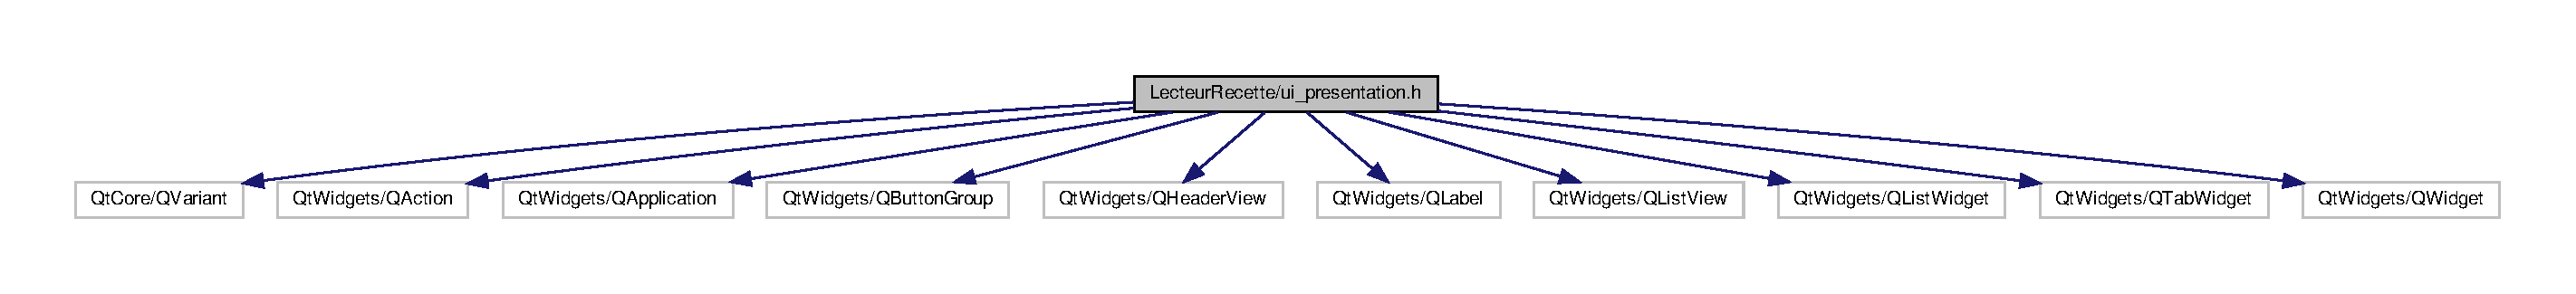
\includegraphics[width=350pt]{ui__presentation_8h__incl}
\end{center}
\end{figure}
Ce graphe montre quels fichiers incluent directement ou indirectement ce fichier \+:
\nopagebreak
\begin{figure}[H]
\begin{center}
\leavevmode
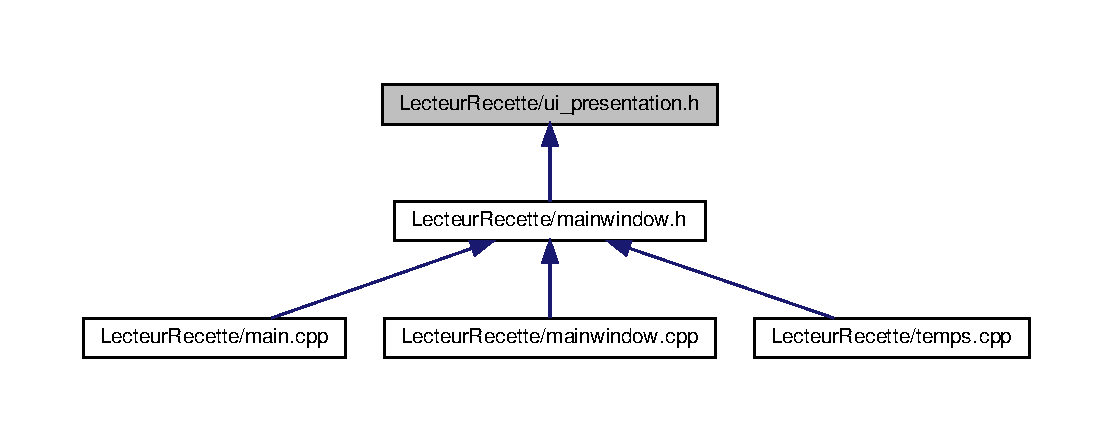
\includegraphics[width=350pt]{ui__presentation_8h__dep__incl}
\end{center}
\end{figure}
\subsection*{Classes}
\begin{DoxyCompactItemize}
\item 
class \hyperlink{class_ui___fenetre_presentation}{Ui\+\_\+\+Fenetre\+Presentation}
\item 
class \hyperlink{class_ui_1_1_fenetre_presentation}{Ui\+::\+Fenetre\+Presentation}
\end{DoxyCompactItemize}
\subsection*{Espaces de nommage}
\begin{DoxyCompactItemize}
\item 
 \hyperlink{namespace_ui}{Ui}
\end{DoxyCompactItemize}

%--- End generated contents ---

% Index
\backmatter
\newpage
\phantomsection
\clearemptydoublepage
\addcontentsline{toc}{chapter}{Index}
\printindex

\end{document}
